\section{The {\systemname} Sleep Monitoring Platform}\label{Sec:2design}

{\systemname} is a novel smartwatch-based sleep monitoring system that aims at estimating sleep quality and capturing rich information
about behaviors and events occurring during sleep. By capturing this information, {\systemname} can analyze potential reasons for sleep
problems and provide the user with suggestions on how to improve their sleep routine or sleep environment. To achieve its design goals,
{\systemname} exploits a wide range of sensors that are common on commercial off-the-shelf smartwatches: (i) the accelerometer, the
gyroscope, and the orientation sensor are used to collect body and hand movements; (ii) the microphone is used to measure the level of
ambient noise and to capture acoustic events; and (iii) the ambient light sensor is used to monitor illumination within the sleep
environment. Table~\ref{tab:test} summarizes the sleep events that can be detected by \systemname using data collected from these sensors.

It is to note that the design choices and algorithm parameters of \systemname are empirically determined from our pilot study
(Sec.~\ref{sec:trainingdata}). The users involved in the pilot study are different from those participating in the experiments for evaluating the developed system (Sec.~\ref{sec:evalusers}).


\subsection{Detecting Sleep Postures and Movements}

One's sleeping position, referred to as {\em sleep posture}, and the extent of body movements are important factors in determining overall
sleep quality. Suboptimal posture has been shown to affect the severity of sleep disorders and is widely used in medical diagnoses to
analyze effects of sleep disorders~\cite{oksenberg1998effect,eiseman2012impact} while having a good sleep posture has been shown to
correlate with subjective assessments of sleep quality~\cite{dekoninck83sleep}. Similarly, the high degree of body movements during sleep
likely reflects restlessness, which results in poor sleep quality. {\systemname} uses motion sensors (accelerometer, gyroscope, and
orientation sensor) to capture the user's sleep posture and habits. In the following, we detail the techniques we use for capturing the
body posture and movements.  {\systemname}, currently supports the four basic sleep postures (see Fig.~\ref{fig:BodyPosture}); three hand
positions (see Fig.~\ref{fig:HandPosition}); six types of body rollovers (see Fig.~\ref{fig:BodyRollover} for an example); and three types
of body micro movements.

\begin{figure*}[!t]
	\centering
	\begin{minipage}[t]{.33\textwidth}
		\centering
		  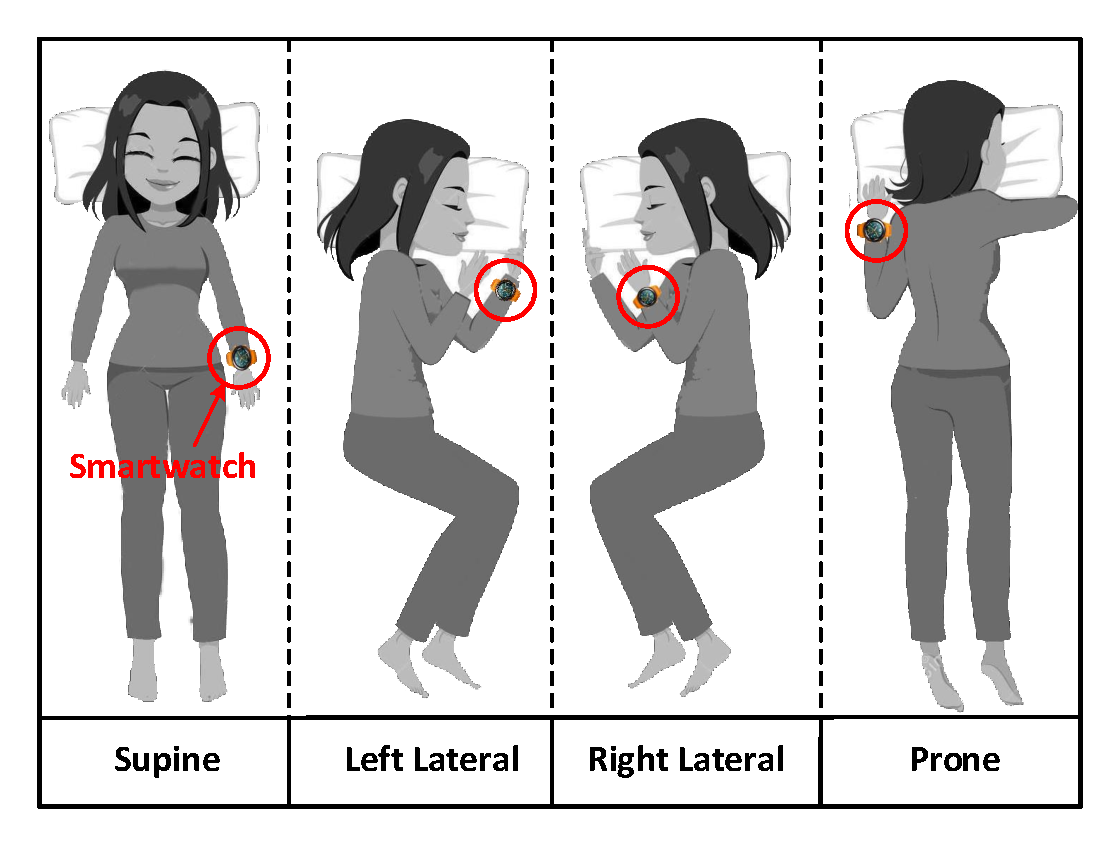
\includegraphics[width=4.7cm,height=3.7cm]{Figures/BodyPosture.pdf}
		\caption{Four sleep body postures.}
		\label{fig:BodyPosture}
	\end{minipage}%
	\begin{minipage}[t]{.33\textwidth}
		\centering
		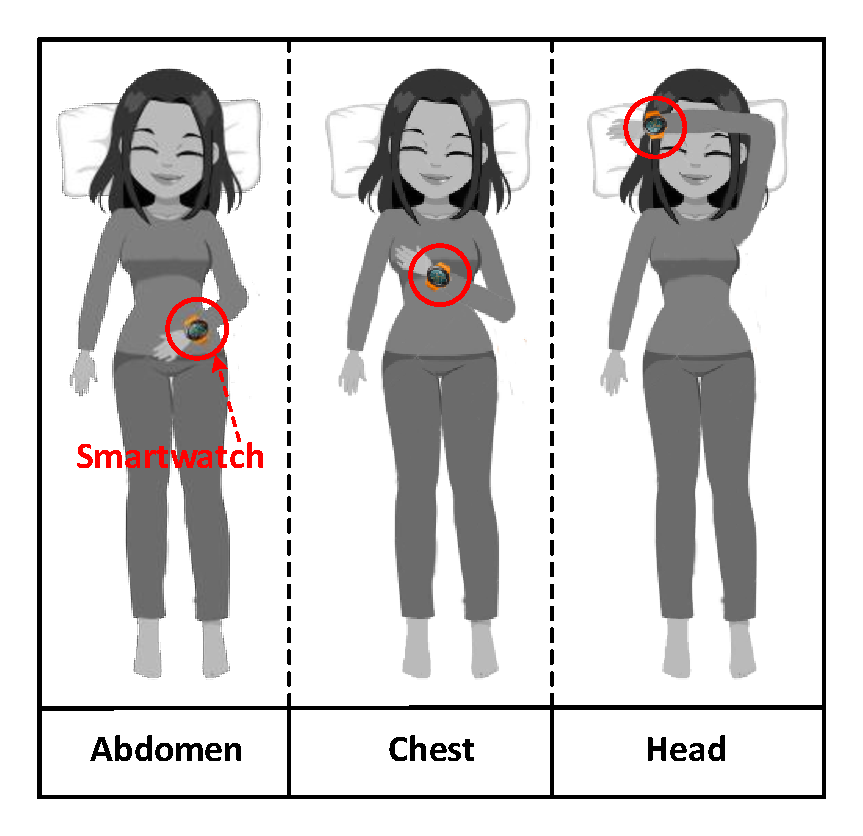
\includegraphics[width=4.1cm,height=3.4cm]{Figures/HandPosition.pdf}
		\caption{Three hand positions.}
		\label{fig:HandPosition}		
	\end{minipage}
\begin{minipage}[t]{.33\textwidth}
		\centering
	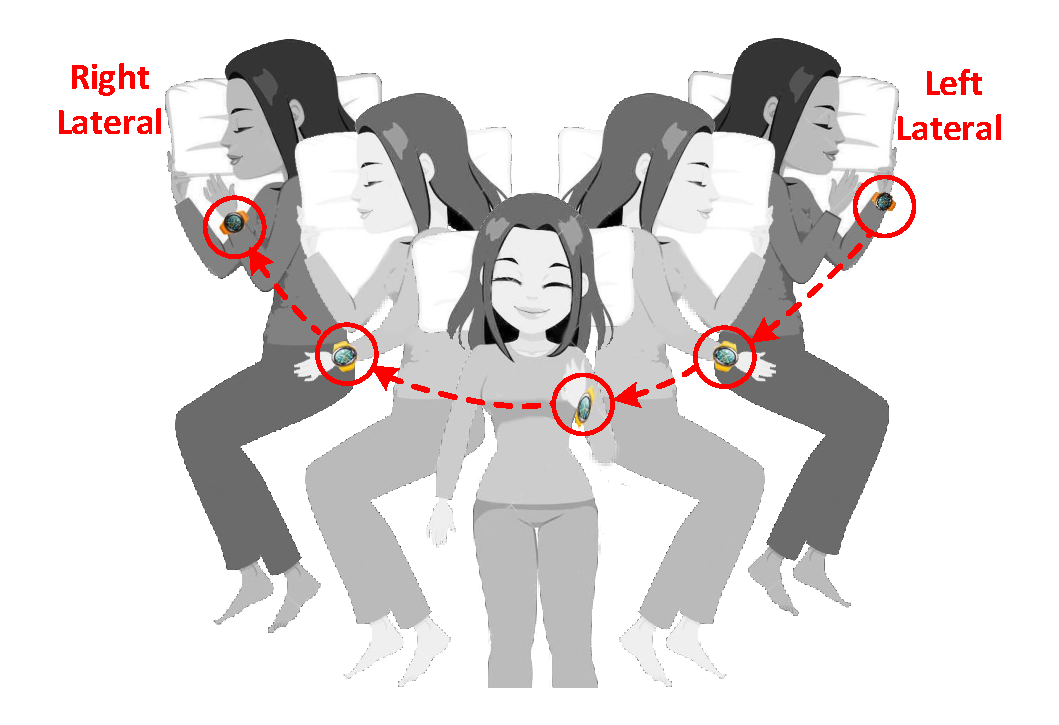
\includegraphics[width=4.7cm,height=3.7cm]{Figures/BodyRollover.pdf}
	\caption{Body rollover from the left side to the right side.}
	\label{fig:BodyRollover}
\end{minipage}
\end{figure*}



\subsubsection{Sleep Posture Detection}\label{sec:sleeppdet}

Dreaming and sleep quality are associated with underlying brain functions, which in turn are affected by body posture~\cite{posture2004}.
Sleep posture also varies across individuals and should fit the personal and physical needs of the individual~\cite{posture2016,posture2017}.
For example, sleeping in a prone position is unsuitable for people with ailments, such as heart disease or high blood pressure. On the
other hand, people can {unconsciously} avoid postures that would be beneficial for health and sleep quality~\cite{posture2015}. Having an
effective way to detect current posture and track changes in it would thus be essential for estimating overall sleep quality, and avoiding
potential harm. {{\systemname} captures four basic sleep postures: supine, left lateral, right lateral, and prone. These are illustrated
in} Fig.~\ref{fig:BodyPosture}. Detecting these postures using a single wrist sensor, however, is non-trivial because the sensor cannot
accurately track the movement of the entire body. To accomplish posture detection, we observe that the arm position strongly correlates {with}
sleep posture, i.e., the arm is typically located in a specific, stable location for a given posture. This suggests that we can first
identify the user's arm position and the {\em time the position is approximately stable, which can then be mapped into} a sleep posture.
Later in this paper, we show that our approach {achieves} high accuracy in identifying sleep postures.

To separate sleep postures, {\systemname} considers a set of feasible hand positions for each posture. {In the supine position, we assume
the user's hand is placed on the left side of the body, on the abdomen, on the chest or on the head; on the left and right lateral
positions we assume the hand to be close to the pillow, on the chest or on the waist; and, finally, in the prone position we assume the
user's hand is on the side of the head or above his/her head.} These positions were selected based on a pilot carried out in our test
environment (see Sec.~\ref{sec:expsetup}). Fig.~\ref{fig:BodyPosture} shows one possible hand position for each of the postures.

Like SleepMonitor~\cite{sleepmonitor}, we use {three dimensional tilt angles} to detect postures. To identify {which posture the data
collected within a time window corresponds to}, we average all the calculated tilt angle values of that window in each dimension. We then
calculate the Euclidean distance of the input values to a set of posture profiles, which are based on measurements collected in a pilot
study that involved 10 users (see Sec.~\ref{sec:trainingdata}). We then use the body posture associated with the nearest neighbor as the
detection outcome. Fig.~\ref{fig:posture} shows the angle values of the four sleep postures targeted in this work. {We can observe clear
differences in the tilt angles of the three axes}. The sleeping posture thus can be inferred based on the position of the smartwatch and the
created angle mapping. However, a limitation of this approach is that the hand positions during supine and prone postures {can be} similar
when the hand is located on the side of the head (Fig. \ref{fig:Supine} and \ref{fig:Prone}), thus the classification accuracy will be
affected.

\begin{figure*}[!t]
	\centering
	\subfigure[Supine]{
		\label{fig:Supine}
		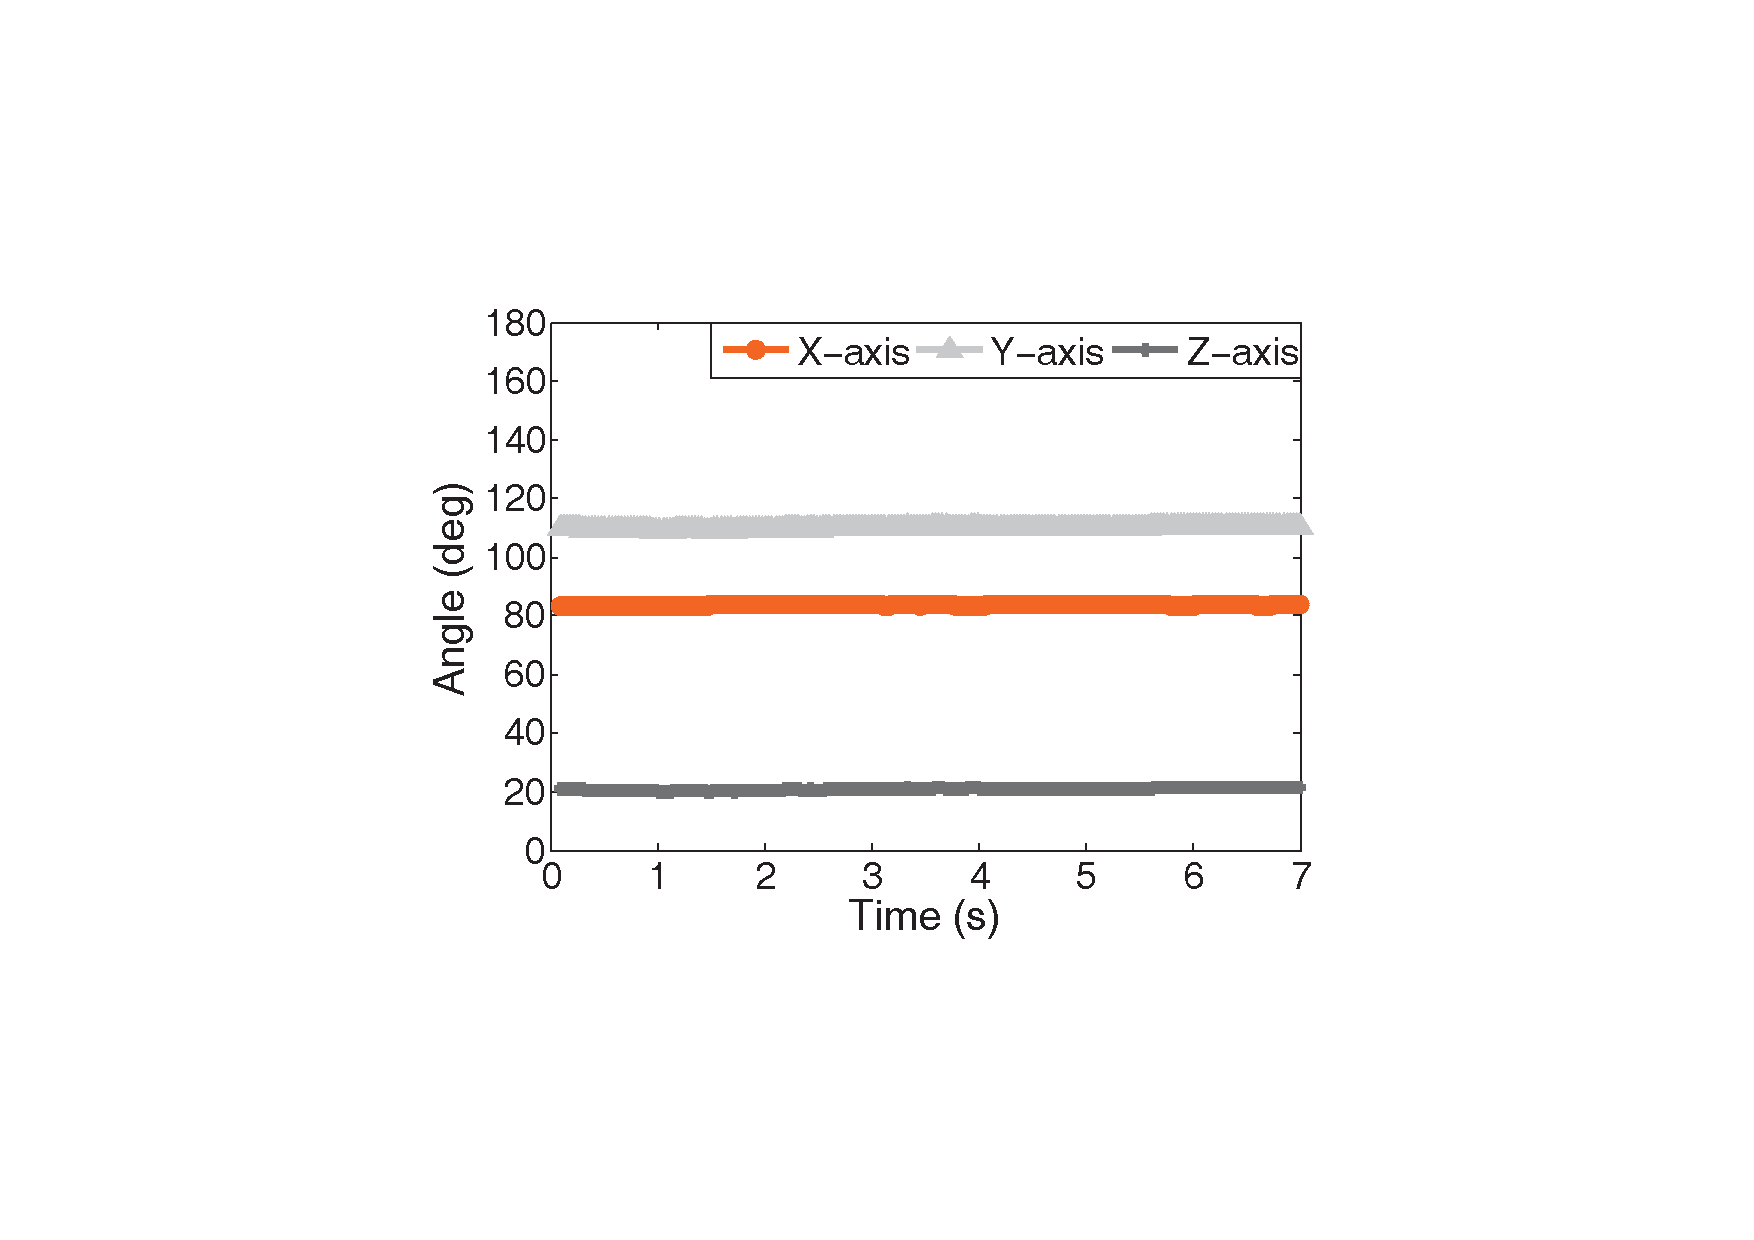
\includegraphics[width=0.237\columnwidth]{Figures/Supine.pdf}}
	\subfigure[Left Lateral]{
		\label{fig:LeftLateral}
		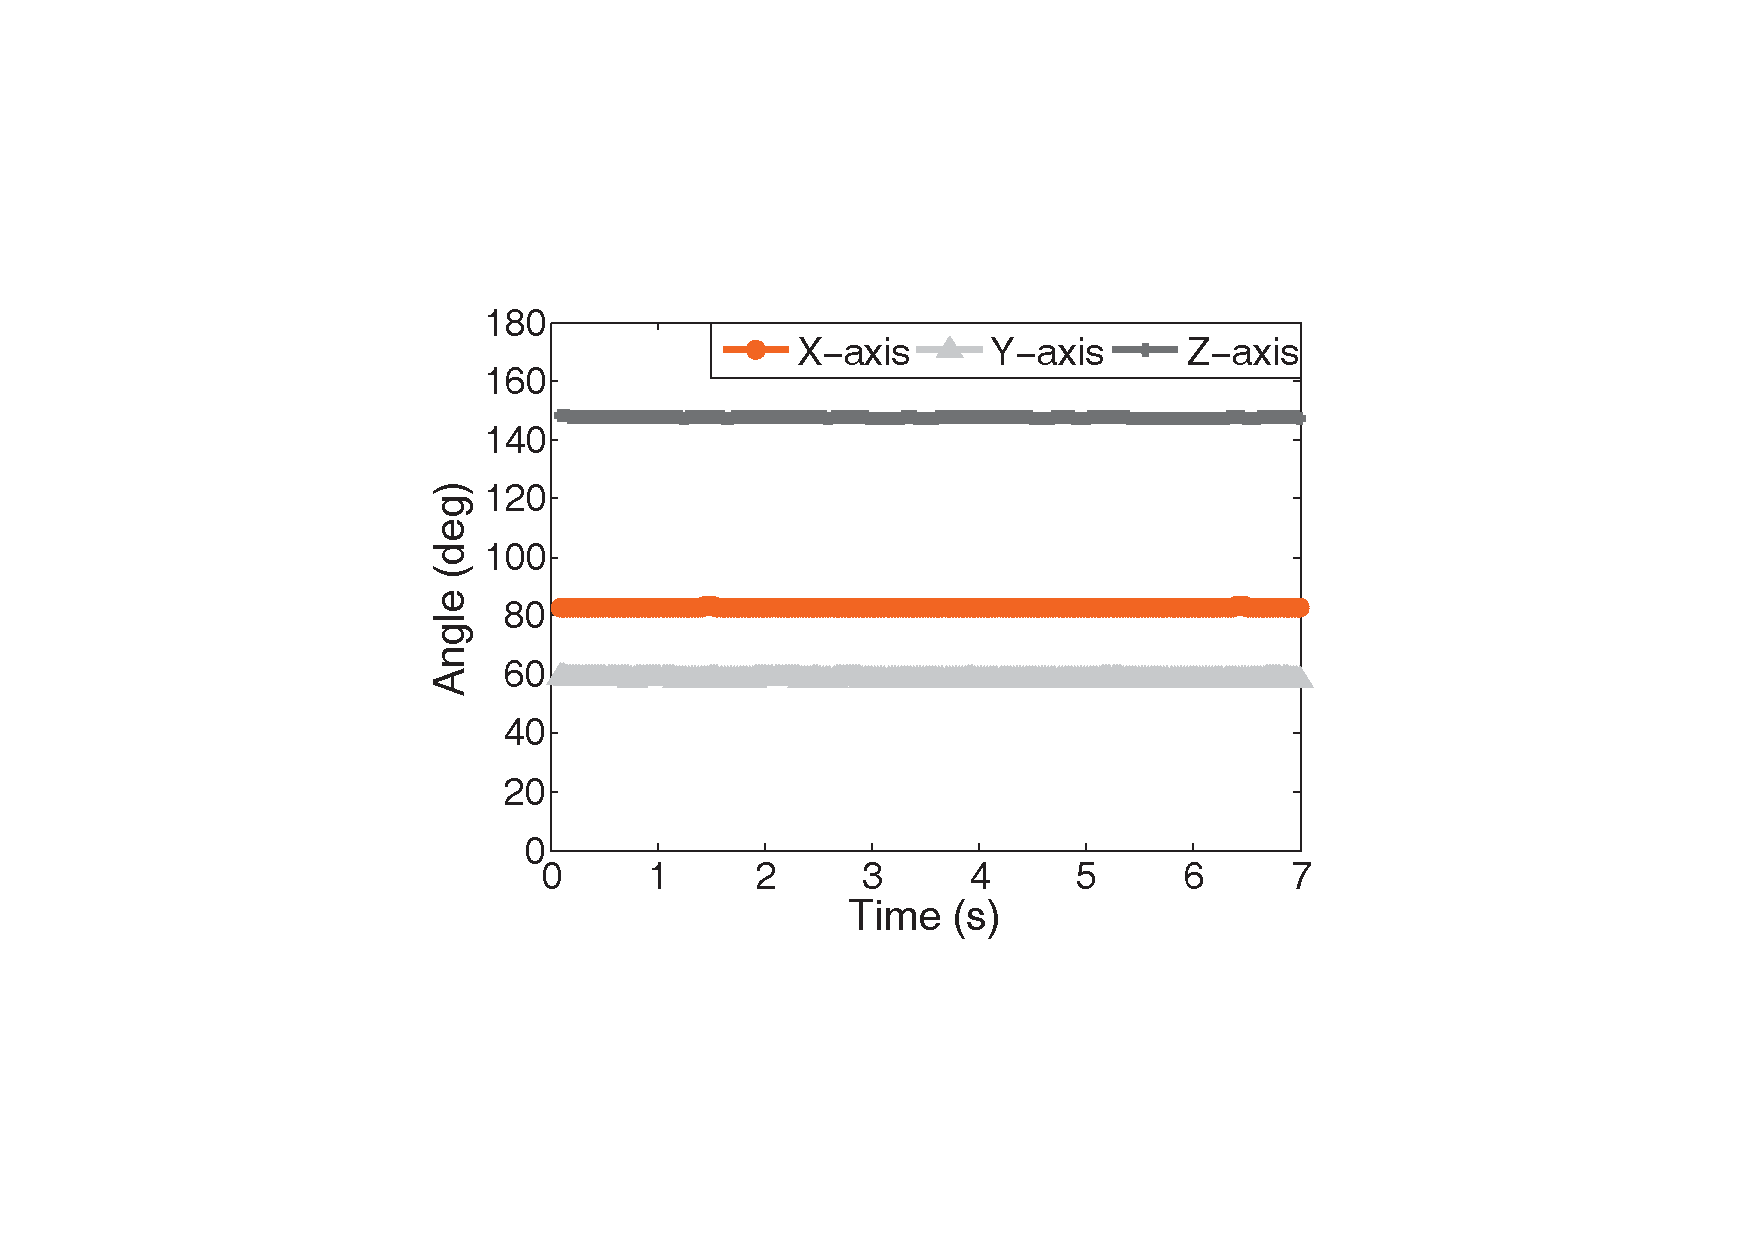
\includegraphics[width=0.237\columnwidth]{Figures/LeftLateral.pdf}}
	\subfigure[Right Lateral]{
		\label{fig:RightLateral}
		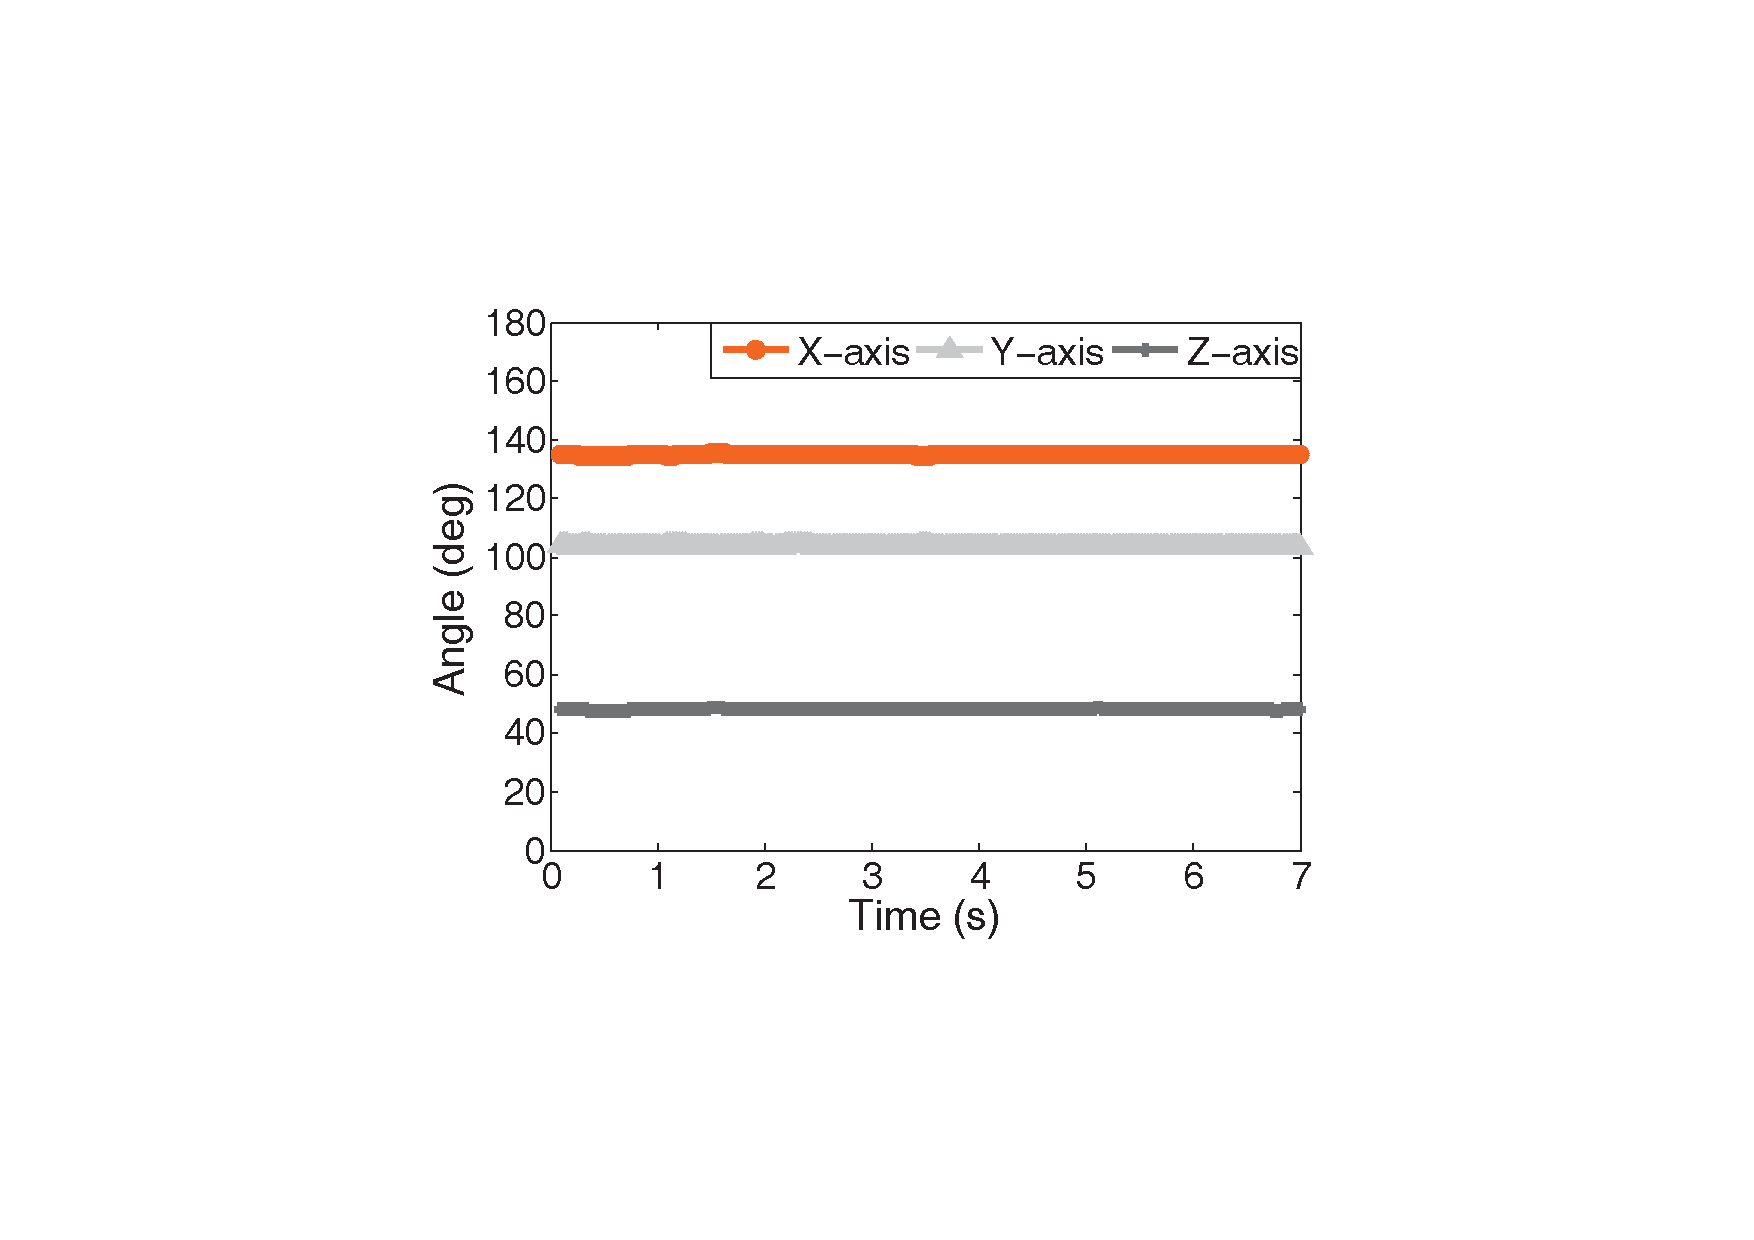
\includegraphics[width=0.237\columnwidth]{Figures/RightLateral.pdf}}
	\subfigure[Prone]{
		\label{fig:Prone}
		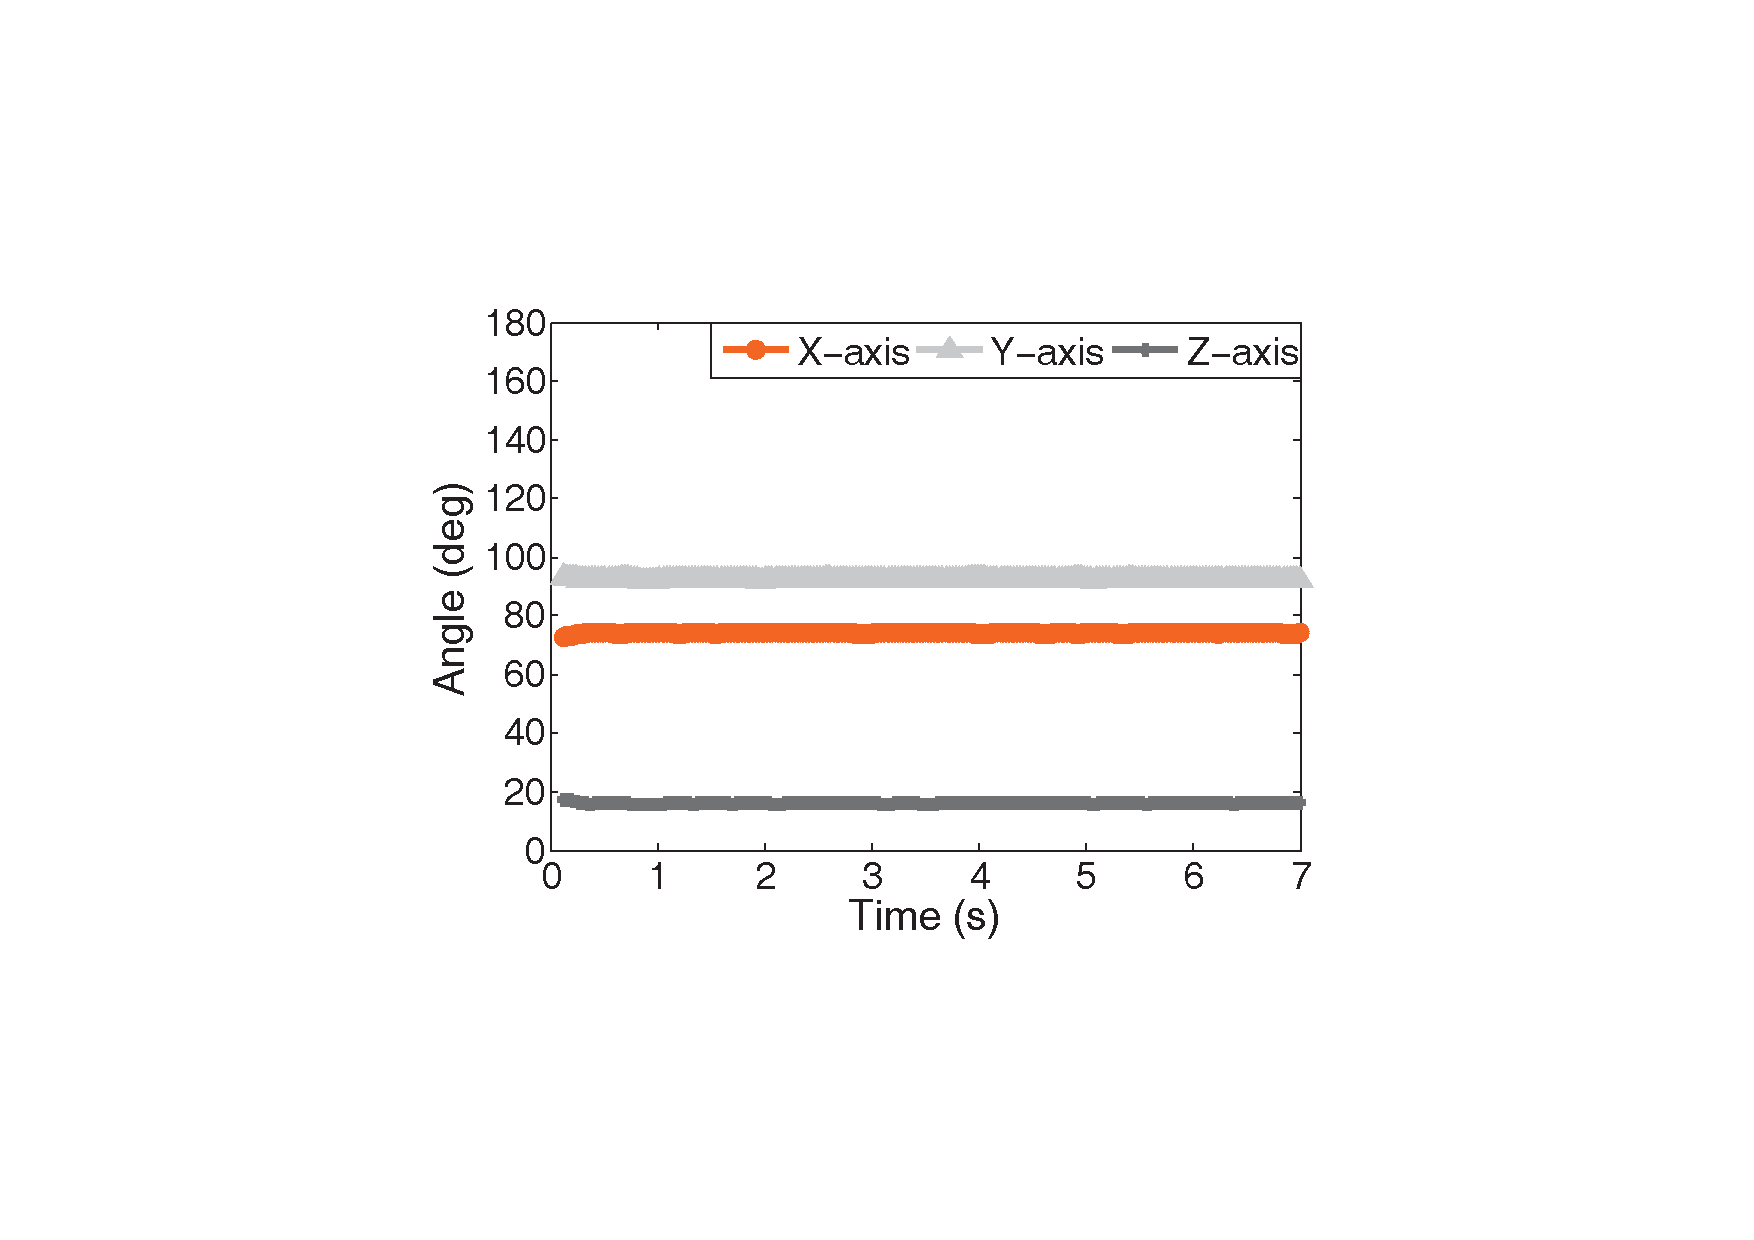
\includegraphics[width=0.237\columnwidth]{Figures/Prone.pdf}}
	\caption{The tilt angle characteristics of four body postures.}\label{fig:posture}
\end{figure*}


To improve detection accuracy between supine and prone postures, {\systemname} integrates orientation data as an auxiliary feature. This is {motivated by the observation that hand directions differ in supine and prone positions}. When the result of the previous step is prone or supine and hand is detected to be located next to the body, we combine the tilt angle with three axes data obtained from the direction sensor as a new feature, and classify these postures using a template-based distance matching approach. Specifically, we return the position corresponding to the template with minimum Euclidean distance with current sensor measurements as the user's posture. When we use the direction sensor, we must limit the pillow orientation remaining unchanged (in the experiment our pillow is placed on the north). In fact, this assumption can be easily satisfied since most people usually have fixed sleep directions.


\subsubsection{Hand Position Recognition\label{sec:handpr}}

The hand position during sleep can disclose potential health problems, and an improper hand position can even result in health issues~\cite{position2014}. For instance, placing the hand on the abdomen may indicate discomfort whereas placing the hand on the chest can increase the likelihood of nightmares due to long-term pressure on the heart. Similarly, placing the hand on the head can put excess pressure on shoulder nerves and cause arm pain as blood flow is restricted. This can lead to eventual nerve damage, with symptoms including a tingling sensation and numbness \cite{position2014}.


{\systemname} is designed to recognize three common hand positions -- if the hand is placed on the abdomen, chest or head when the user is in the supine posture, as shown in Fig. \ref{fig:HandPosition}. We have chosen these three hand positions because there are found to be the most common and representative positions in our pilot study (Sec.~\ref{sec:trainingdata}). Our hand position recognition algorithm is based on sensor data of rotation angles, tilt angles, and respiratory events. It works by first using the rotation and tile angles to detect if the hand was placed on the head. {When the hand is not on the head, we use respiratory events to identify whether the hand is on the abdomen or chest}. We now describe how to detect each of the three positions in more details.


\cparagraph{Hands on the head.}  Fig.~\ref{Bodyhand} shows the change of rotation angle using the gyroscope for one of our pilot study users
when his hand was initially placed next to the body and then moved to his head, abdomen, and chest. As can be seen from the figure, when
the hand is moved to the head, changes in rotation angles are significantly different from the readings when moving the hand on the abdomen or
chest. This is largely due to the palm facing direction - it is upward when the hand is placed on the head but downward when the hand is
placed in other positions. {\systemname} exploits this observation to detect if the hand is placed on the head by examining changes of the
{tilt} and rotation angles. We use a hierarchical classifier consisting of two {K nearest neighbor} models (with $K=1$) to predict if the
hand is moved to the head based on the tilt and rotation angle readings. Specifically, we use the first KNN model to detect if the input
tilt angle reading is closest to one of our training samples where the palm was {facing up. Training data for detecting palm direction
(upward or downward) are collected} from our pilot study users when their hands are placed on the head, abdomen and  chest respectively;
see Sec.~\ref{sec:trainingdata}) If the first KNN model suggests that the palm was facing upward, the second KNN then uses differences of
rotation readings (from the x, y, and z directions) before and after hand movement to determine if the most likely position is on the head
or elsewhere. As similarity measure we consider the  Euclidean distance from the input data to each of the training samples -- consisting
of the rotation angle values from the three directions. If our hierarchical model predicts that the hand was not placed on the head, we
then use the method described in the next paragraph to detect if it was placed on the abdomen or the chest.

\begin{figure*}[!t]
	\centering
	\subfigure[moving to the head]{\label{BodytoHead}
		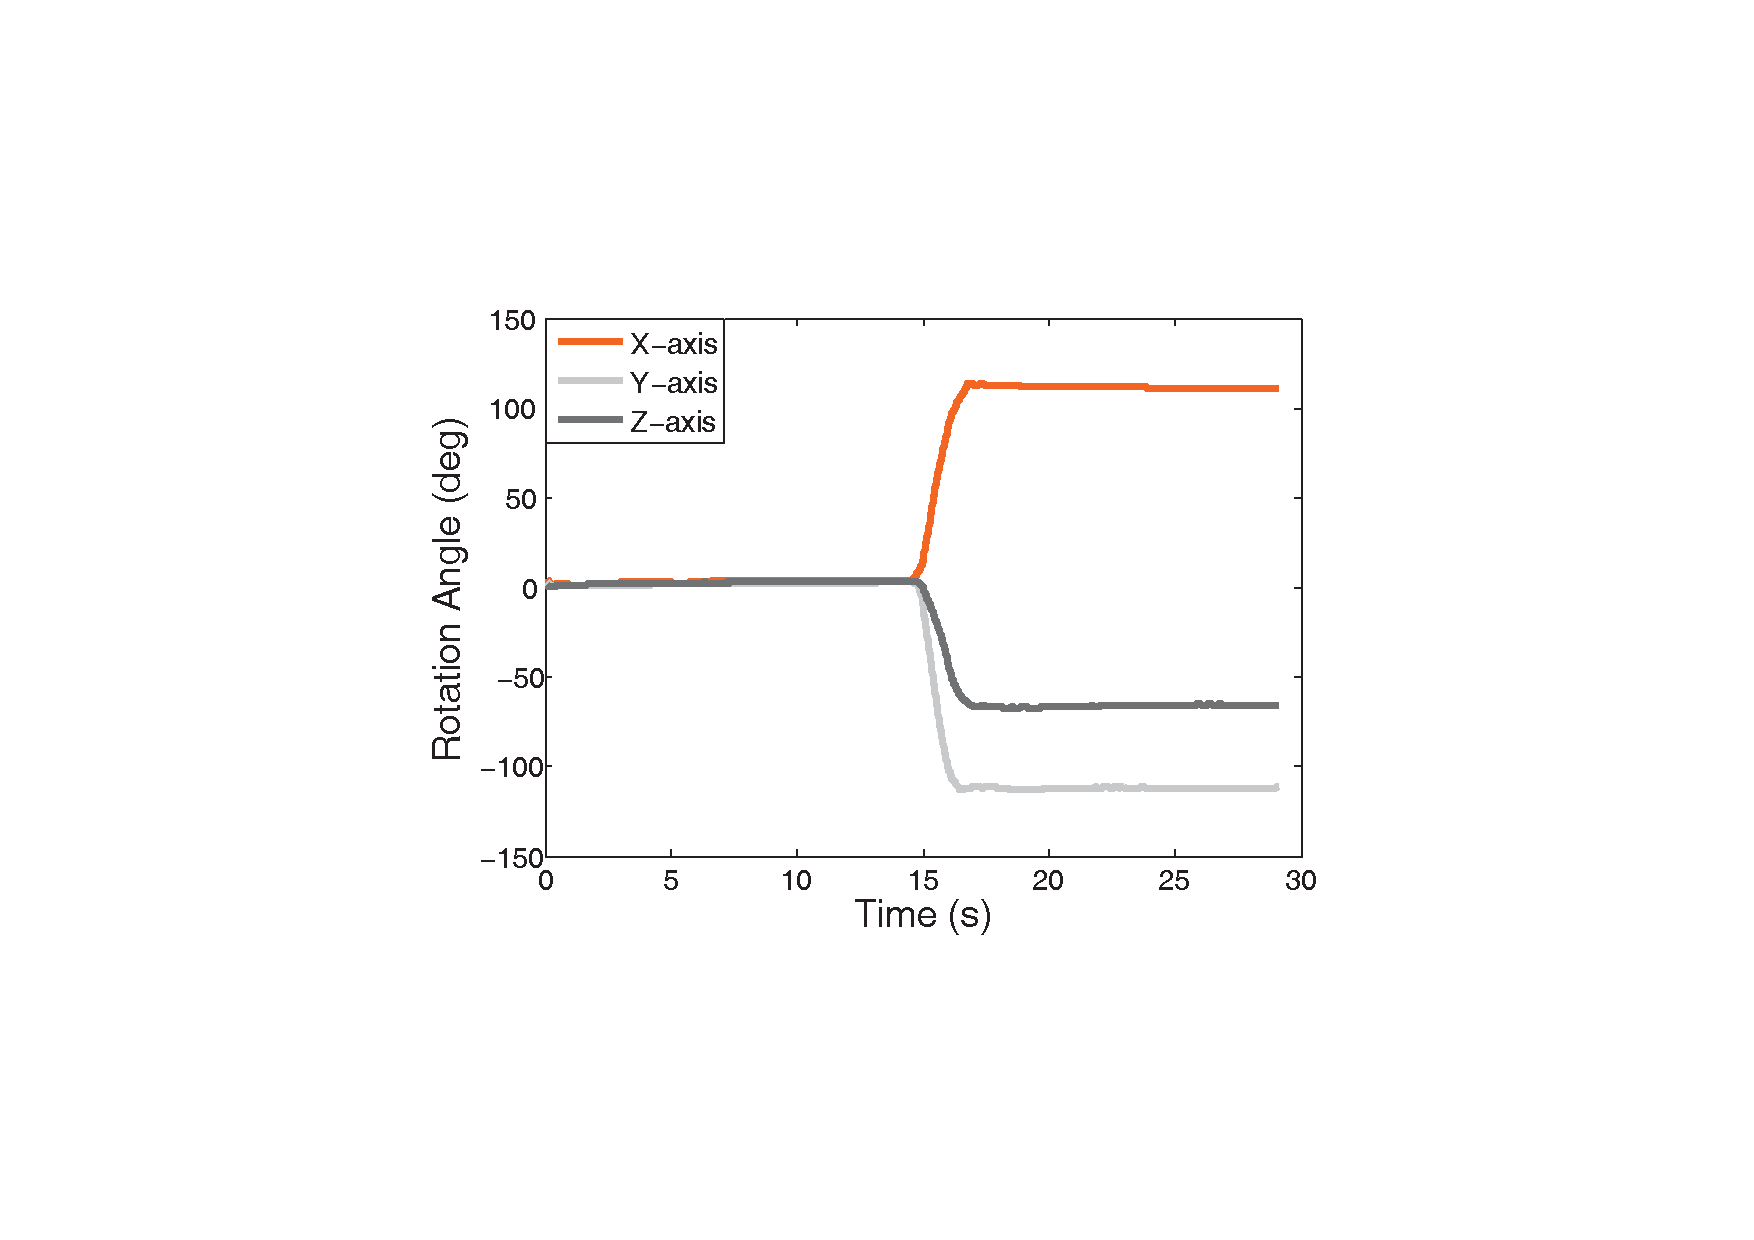
\includegraphics[width=0.32\linewidth]{Figures/BodytoHead.pdf}}
	\subfigure[moving to the abdomen]{\label{BodytoAbdomen}
		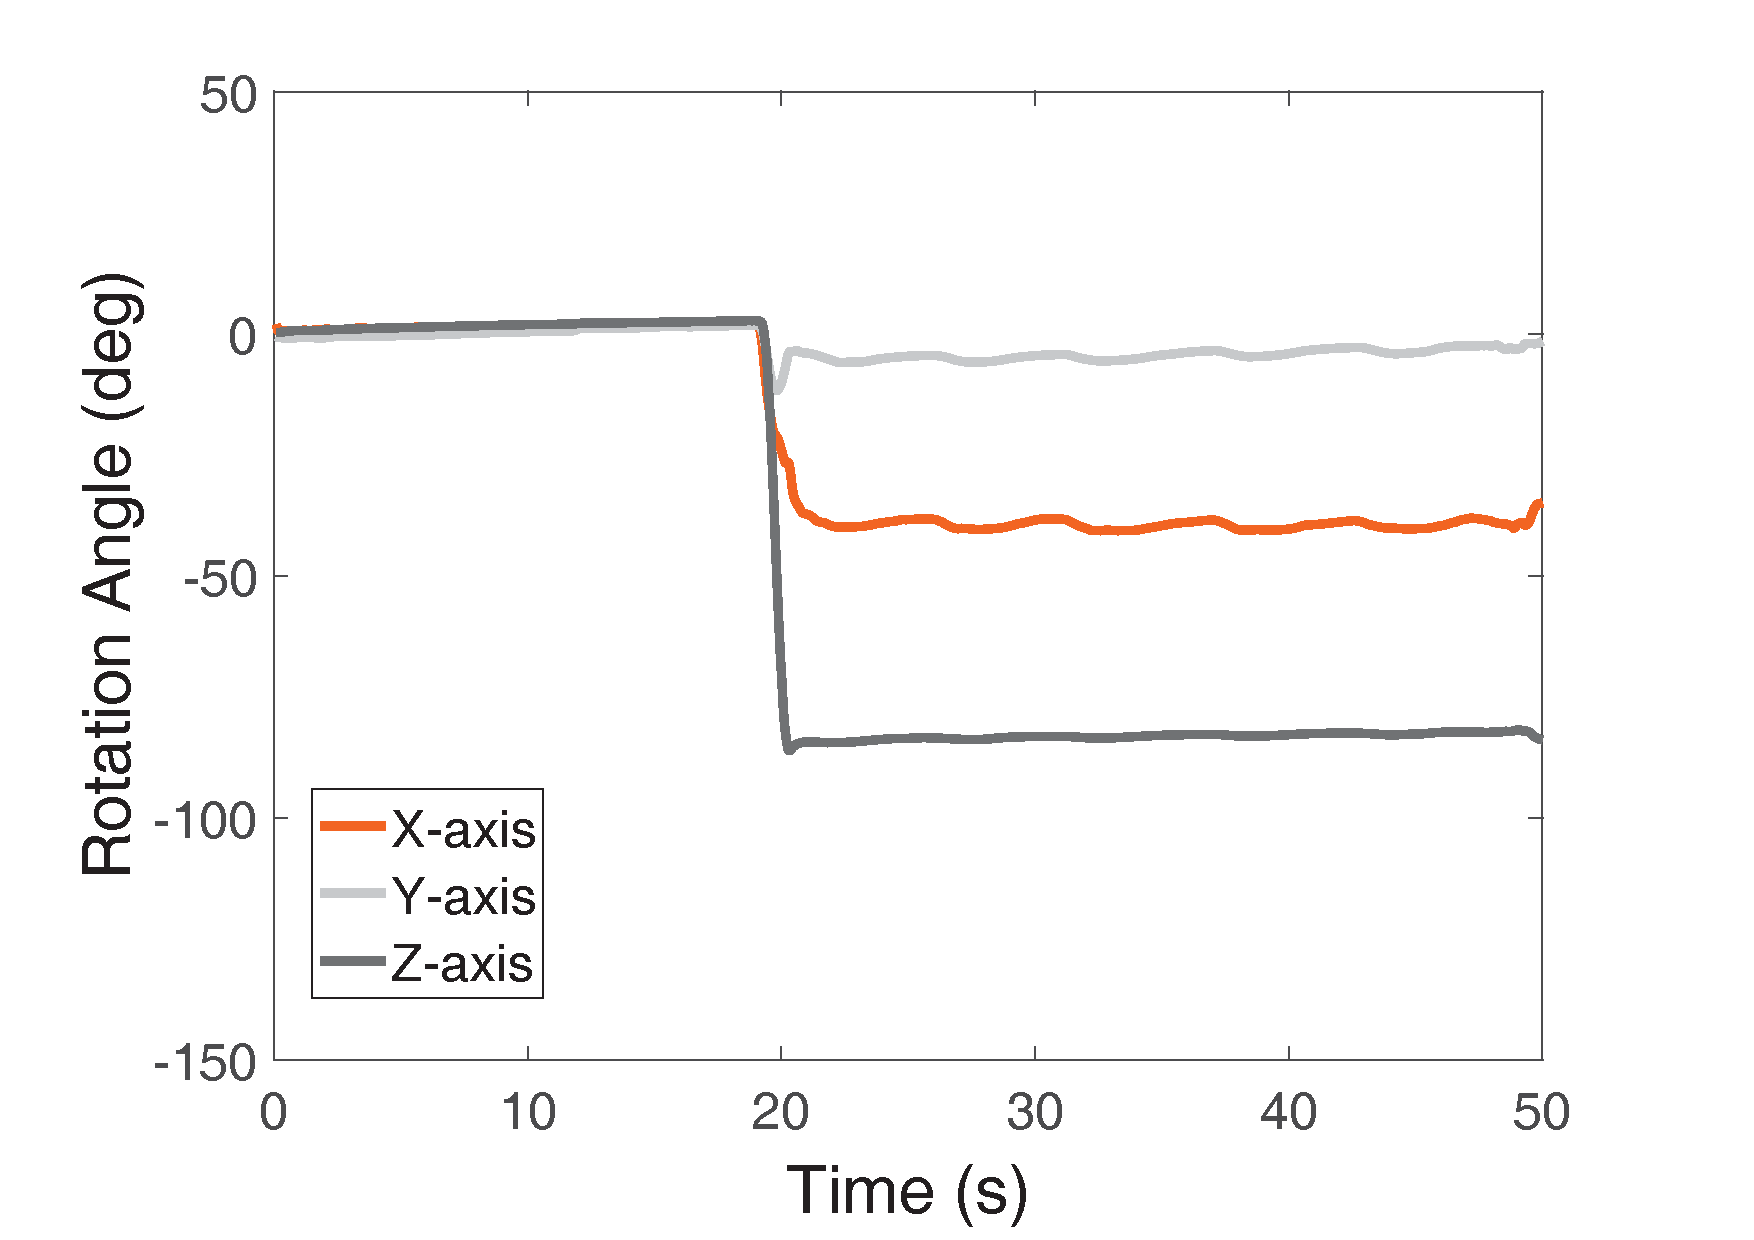
\includegraphics[width=0.32\linewidth]{Figures/BodytoAbdomen.pdf}}
	%  \hfill
	\subfigure[moving to the chest]{\label{BodytoChest}
		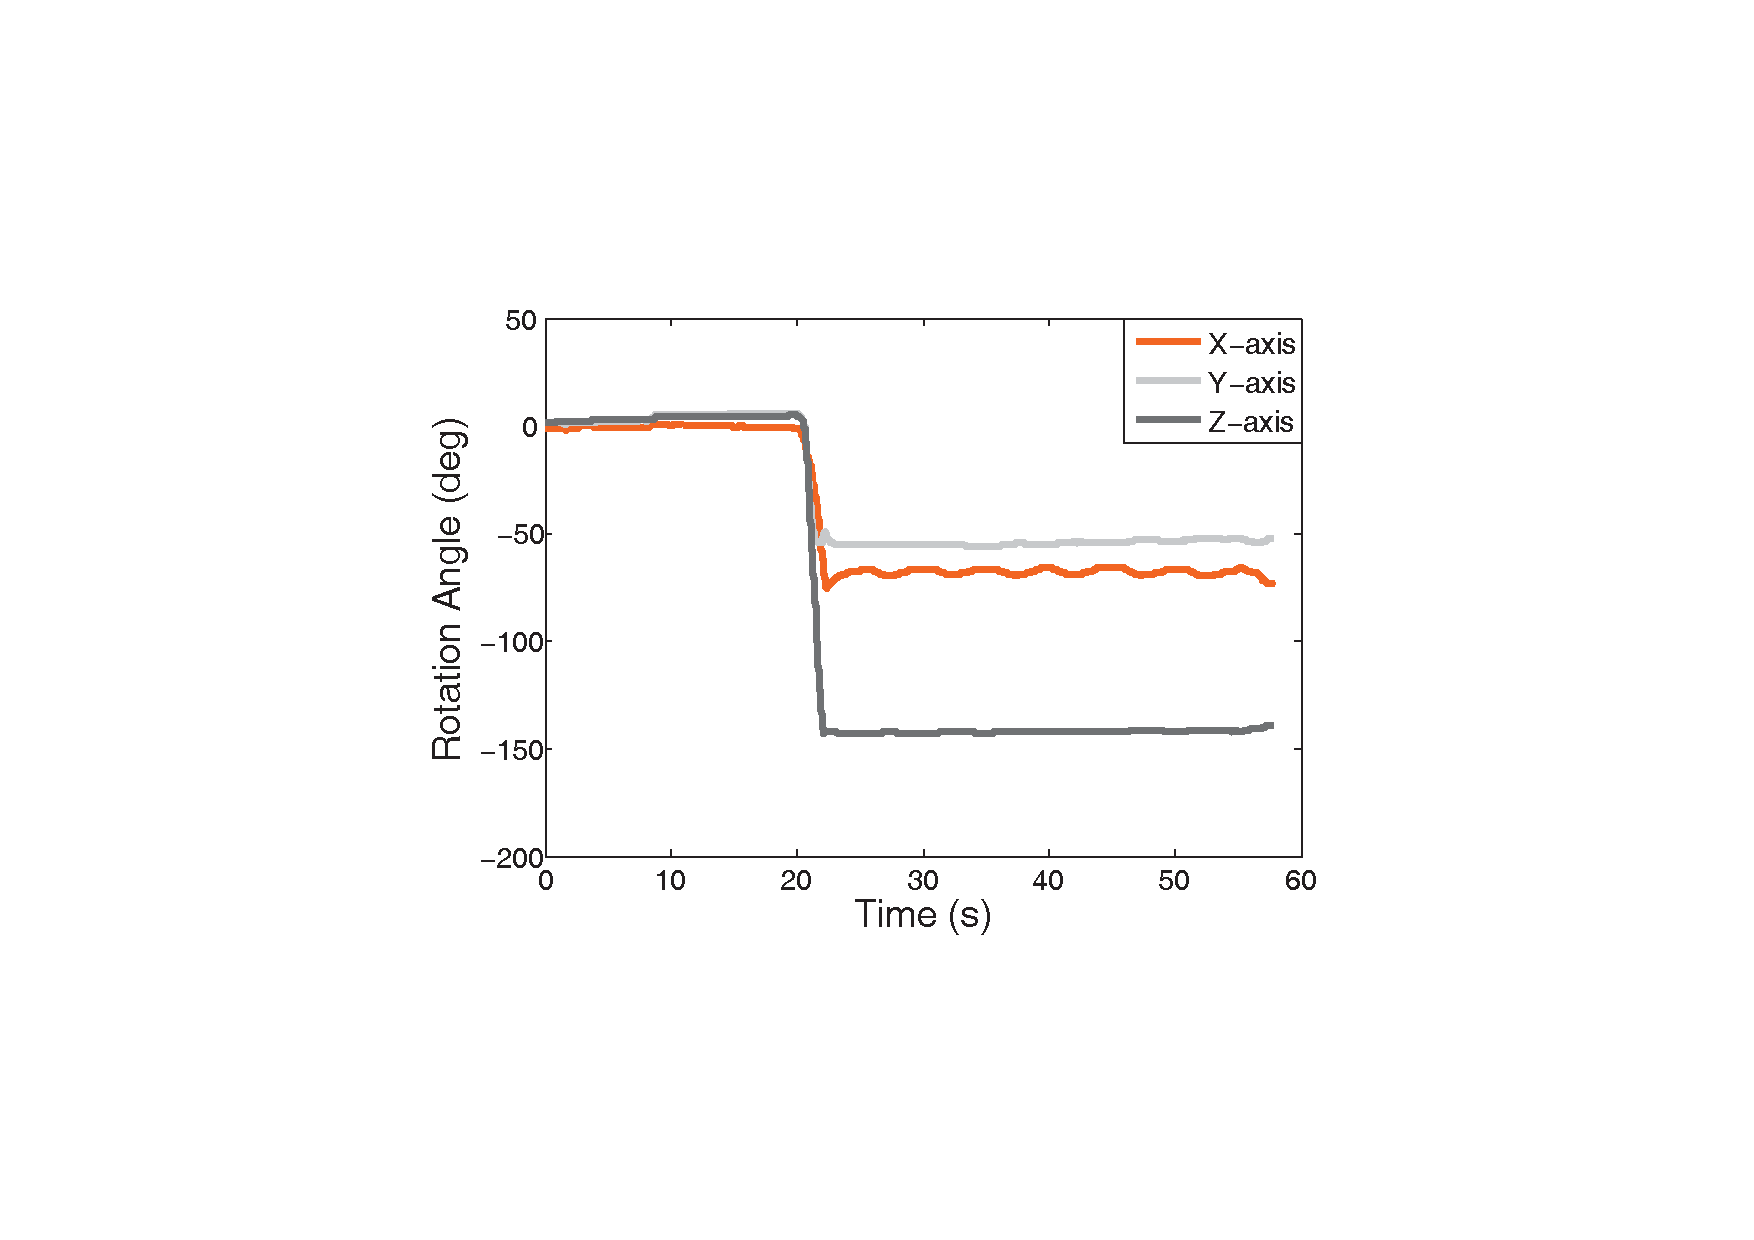
\includegraphics[width=0.32\linewidth]{Figures/BodytoChest.pdf}}
	\caption{The differences of the rotation angle when a hand of one of our users, placed next to the subject's body, is moved to the subject's head (a), abdomen (b), and chest (c). }\label{Bodyhand}
\end{figure*}



\cparagraph{Hands on the abdomen or chest.} {When the aforementioned hierarchical model predicts the hand is not placed on the head, the
hand can then be located anywhere, including different parts of the body. {However, in our case we are only interested in detecting if
the hand is on the chest or abdomen -- or at neither of these positions.} We build on the intuition that the hand is likely to be affected
by breathing whenever it is placed on the chest or abdomen.} Specifically, the impact of breathing results in periodical fluctuations on
the accelerometer readings. This is because the hand will be pushed up and drop down due to breathing.  {Our experimental data suggest that
this behavior only takes place when the hand is placed on the abdomen or the chest, not when the hand is located elsewhere (such as the
shoulder). Therefore, we can separate these two locations from others by examining whether the accelerometer values are impacted by
respiration.}

To examine if the accelerometer data are affected by the respiration, we calculate the power spectral density (PSD) of the collected accelerometer data.  {We then check the PSD to see if we can observe any peak that closely matches human respiratory frequency}. A match indicates that the hand is affected by a respiratory event and hence the hand is likely to be placed on either the abdomen or the chest. Fig. \ref{fig:PSD} provides an empirical evidence to support our design choice. It shows the PSD for one of pilot study user when his hand was placed on the chest. Here we calculate the PSD for the accelerometer data collected from the x, y and z directions. We can see from the diagram that there is a large peak located at around 0.25Hz (highlighted in the diagrams) when a respiratory event is detected (which was verified by video feed). This peak corresponds to the average respiratory frequency of an adult (0.2Hz to 0.47Hz)~\cite{Breath_frequence}, suggesting that the PSD reading can be used as a proxy to detect respiratory events. {\systemname} thus exploits the PSD to detect if the hand is placed on the abdomen or the chest by checking if there is any peak value of PSD falls within the range of 0.2Hz (corresponding to 12 breathes per minute) and 0.47Hz (corresponding to 28 breathes per minute).

\begin{figure*}[!t]
	\centering
	\begin{minipage}[t]{.4\textwidth}
	\centering
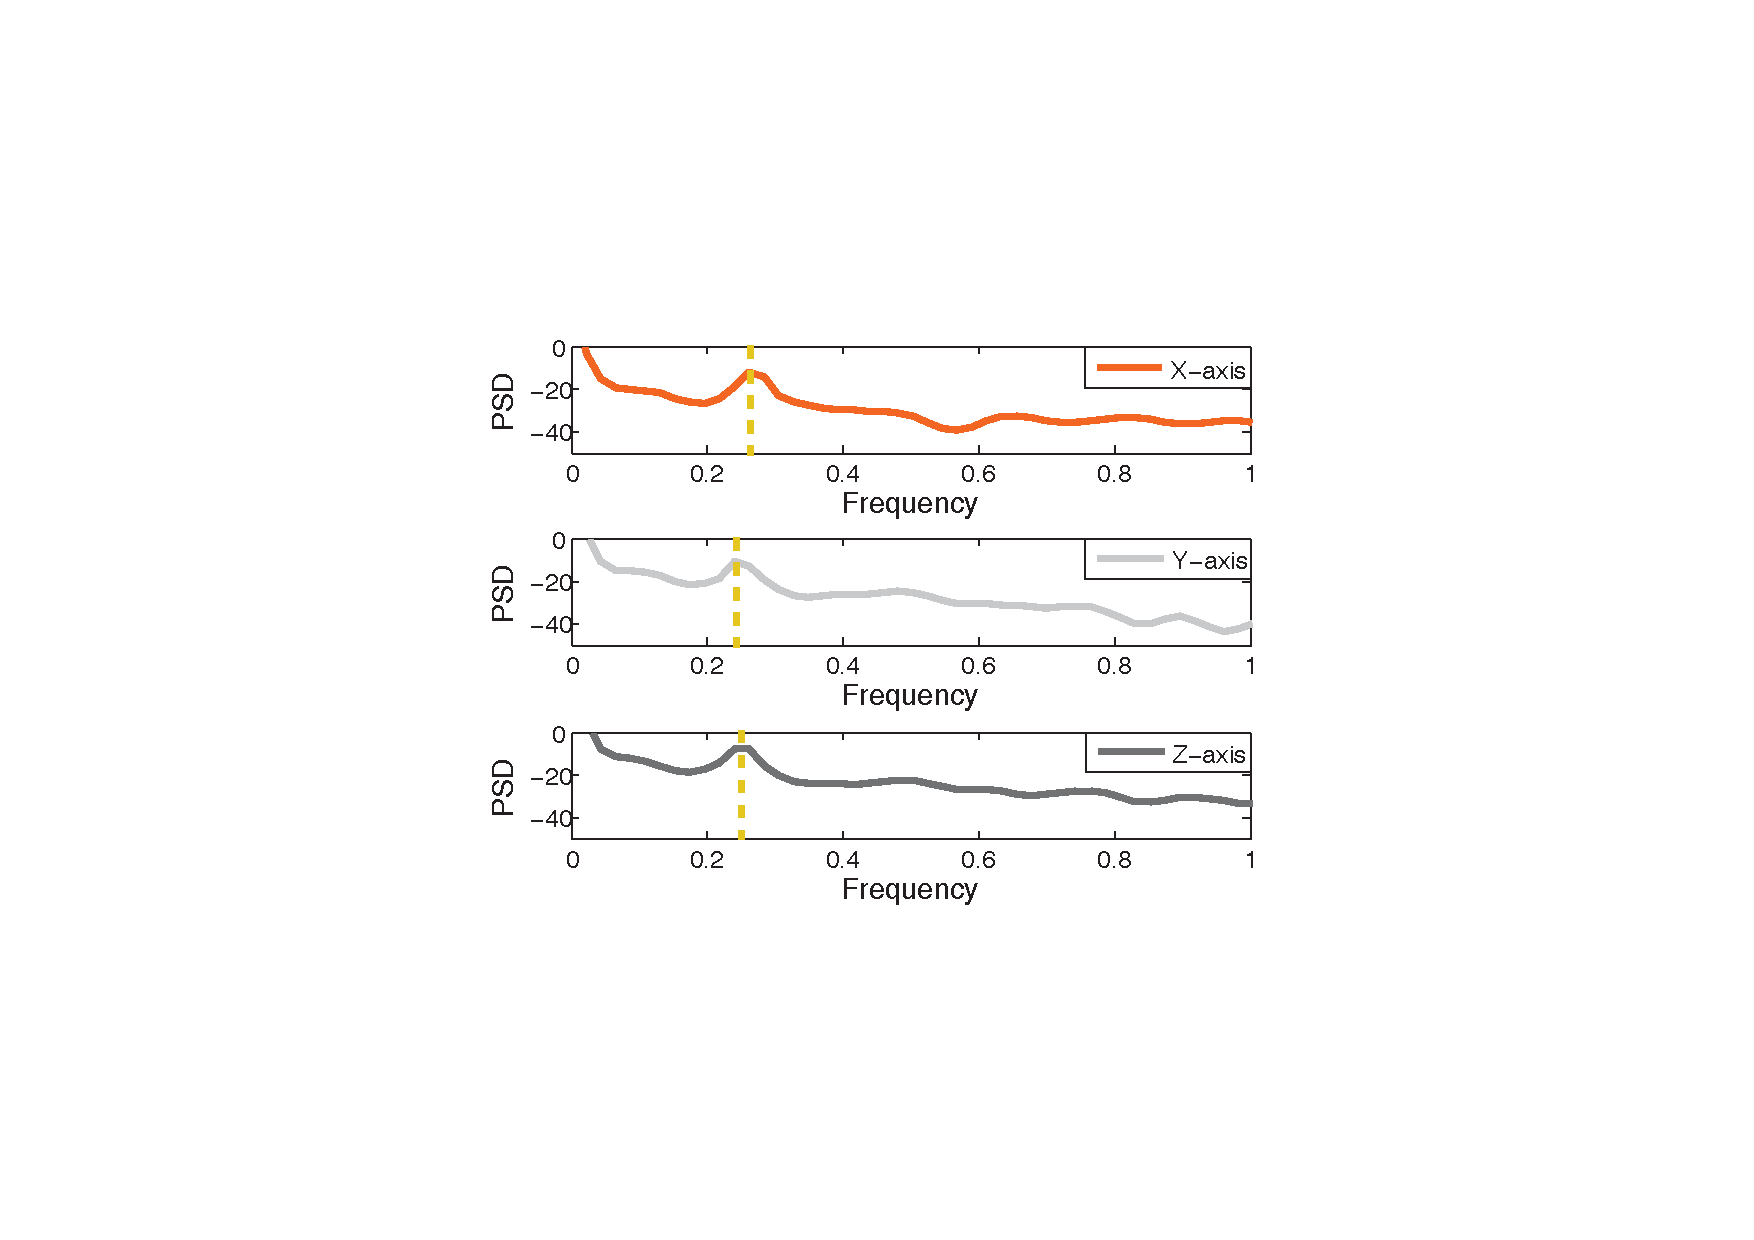
\includegraphics[width=7cm,height=5.7cm]{Figures/PSD.pdf}
\caption{The power spectral density (PSD) of the accelerometer readings when a user's hand is placed on his chest.}\label{fig:PSD}
	\end{minipage}%
\hfill
	\begin{minipage}[t]{.55\textwidth}
	\centering
	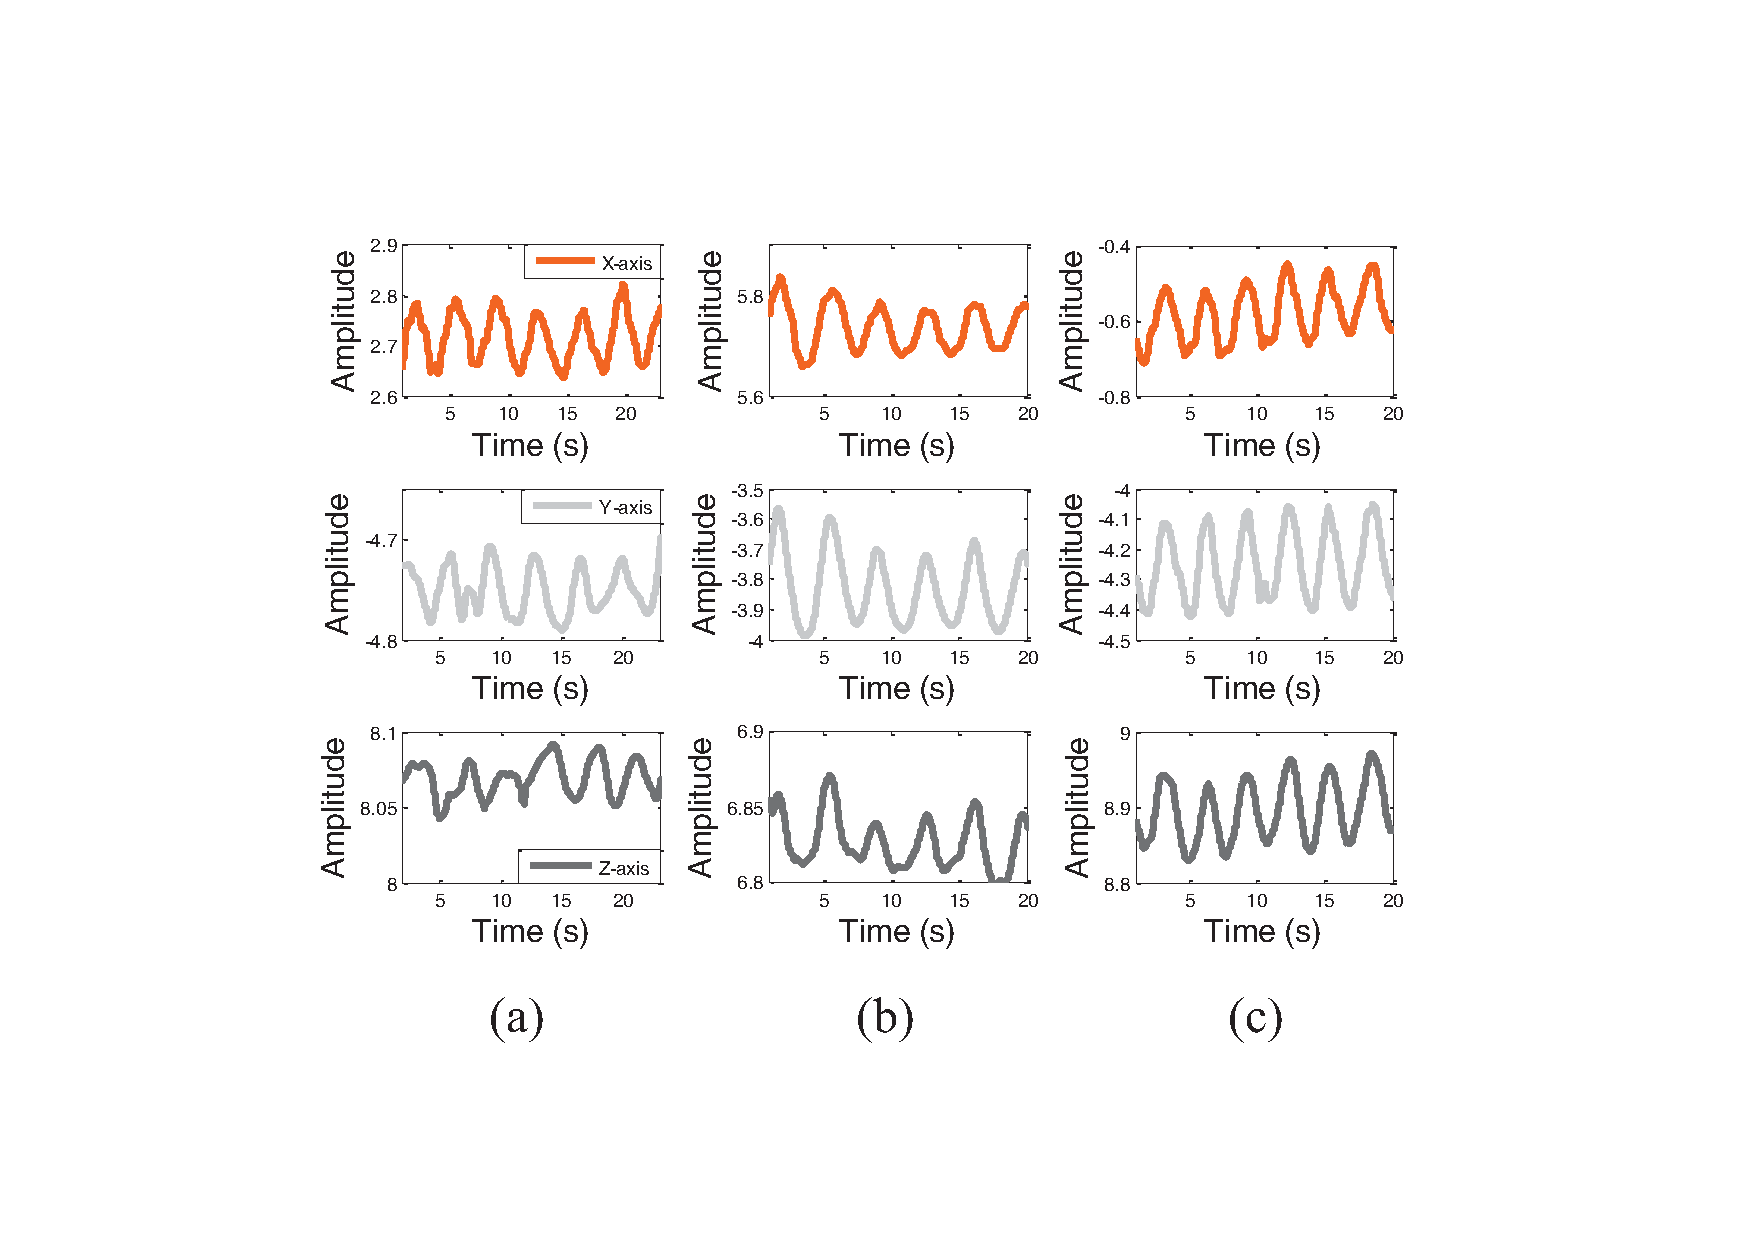
\includegraphics[width=8cm,height=5.7cm]{Figures/breath_ok1.pdf}
	\caption{The periodic change of the acceleration signal. (a) REM--Location 1. (b) REM--Location 2.  (c) NREM--Location 1.}\label{fig:breath_ok1}
	\end{minipage}
\end{figure*}

Putting things together, we thus first use the PSD detector to identify whether a respiratory event is taking place. When respiratory
events are detected, we then use again a KNN classifier to make a binary decision to determine if the hand is placed on the abdomen or the
chest based on the rotation angle readings (see b and c in Fig.~\ref{Bodyhand}). {On the other hand, if no respiratory peak is detected, we
assume the hand to be located at another place on the body that is not supported. } Similarly to the head position model, the training
samples for the KNN model are also collected from our pilot study users -- where each training example includes the rotation angle readings
when the hand is either placed on the abdomen or the chest.

\subsubsection{Labeling REM/non-REM Stages\label{sec:labelrem}}

We have also found that the extent of body movements can be used to judge the amplitude of respiration, which in turns allows us to detect
rapid-eye-movement (REM) and non-rapid-eye-movement (NREM) stages. This is based on a prior study showing that when people sleep in the REM
stage, their respiratory amplitude is smaller than that in the other stages~\cite{respiratory1982}. Hence, we can roughly determine the
user's current sleep stage based on the respiratory amplitude. Respiratory amplitude is only an indicator of the division of the sleep
stage and we can not regard it as a basis for final judgment. {However, it serves as an early reference that helps later phases of the
sleep stage detection. Normally chest movement amplitude is smaller than abdominal movement amplitude. However, during different sleep
stages, respiration amplitudes differ~\cite{respiratory}. Therefore, it is likely that there is a situation where chest movement amplitude
in the NREM stages is close to the abdominal movement amplitude in the REM sleep stage. As a result, a na\"{\i}ve solution of applying a
threshold cannot work satisfactorily but we can combine it with the position of the hand detected earlier. Through the above steps, we have
been able to determine whether the hands are on the chest or abdomen, and then we can go further to determine the extent of breathing
according to the degree of up and down motions, from which we can approximately infer the current sleep stage}.
\begin{figure}[!t]
\centering
      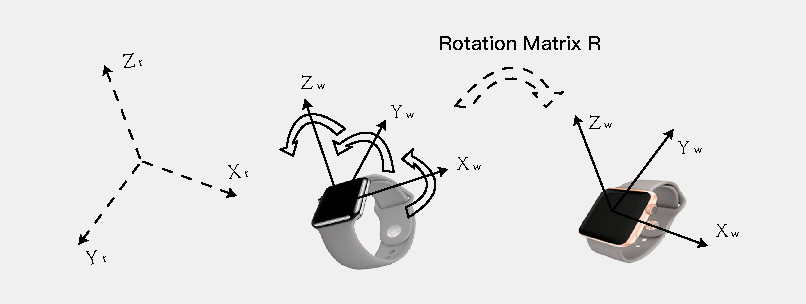
\includegraphics[width=0.67\linewidth]{Figures/watch.pdf}
  \caption{Coordination system conversion. The left-most figure is the torso coordinate system where $Y_t$ points to the north.
  The middle figure shows the watch's coordinate system when the watch is placed on an arbitrary position.
  The right-most figure shows that the resulting watch coordinate system after performing the coordinate system conversion.}\label{fig:watch}
\end{figure}

\cparagraph{Example.} Now we take the case of hands on the abdomen as an example. Even when the hand is placed on the abdomen, there are
some minor changes in the exact location of the user's hand, and the intensity of accelerometer fluctuations caused by respiration also
varies greatly. Hence, we cannot use the amplitude information to determine true respiratory amplitude directly. This problem is
illustrated in Fig.~\ref{fig:breath_ok1}, where (a) and (b) contain triaxial acceleration measurements at different locations of the
abdomen during REM sleep stage, and in (c) which consists of acceleration data for NREM stages at the same approximate position as in (a).
{We can see that when the hand is on the abdomen, but the location differs, we cannot directly judge the respiratory amplitude from the
amplitude of the three accelerometer axes.}

To solve this problem, we convert the acceleration data from the wristwatch coordinate system into the torso coordinate system. {As breathing results in chest moving up and down, movements along the z-axis in the torso coordinate system can be used to identify respiratory amplitude}. We express the tri-axial acceleration data as $Acc_w$ = [$X_w$, $Y_w$, $Z_w$] in the wristwatch coordinate system and $Acc_t$ = [$X_t$, $Y_t$, $Z_t$] in the torso coordinate system, as shown in Fig.~\ref{fig:watch}.  {Our coordinate alignment aims to find a rotation matrix $R$ that aligns the watch's coordinate system with the torso coordinate system ({[$X_t$, $Y_t$, $Z_t$]}). Matrix $R$ can be obtained from the three-axis direction information of the orientation sensor. Specifically, we have:}
\begin{equation}
      X_t  = (X_w {\cos\gamma} + Y_w{\sin\gamma}){\cos\theta} + (Y_w\cos\sigma + Y_w\sin\sigma)\sin\theta,
\end{equation}
\begin{equation}
      Y_t = -((Y_w\cos\sigma + Y_w\sin\sigma)\cos\theta - (X_w\cos\gamma + Y_w\sin\gamma)\sin\theta),
\end{equation}
\begin{equation}
      Z_t = (Z_w\cos\gamma - Z_w\sin\gamma)\cos\sigma - (Z_w\cos\gamma - Z_w\sin\gamma)\sin\sigma,
\end{equation}
where $\theta$, $\sigma$ and $\gamma$ are the x, y and z axis data of the orientation sensor respectively, representing the direction angle, the tilt angle and the roll angle collected from the orientation sensor. After alignment, we can see in Fig.~\ref{fig:cordi} that the z-axis shows a periodic signal with significant fluctuations, {while the x- and y-axis data undergo smaller changes around zero, which is consistent with stable sleep influenced only by respiratory patterns.}

%The two graphs on the left of Fig.~\ref{fig:cordi} show the same acceleration data as has been used in (a) and (c) ofFig.~\ref{fig:breath_ok1}, respectively.
The first graph from the left of Fig.~\ref{cordi0} and Fig.~\ref{cordi1} show the same acceleration data as has been used in \textcolor{red}{(a)} and \textcolor{red}{(c)} of
Fig.~\ref{fig:breath_ok1}, respectively. The two right-most graphs correspond to data after coordinate system alignment.  We can see that,
prior to alignment, we cannot effectively distinguish the respiratory amplitude of REM and NREM stages from the acceleration amplitude.
After coordinate alignment, the respiratory amplitudes are clearly visible from the z-axis data. {To separate REM and NREM stages,} we
calculate the variance of z-axis acceleration and use it as a feature to measure the intensity of the fluctuation in a signal, with larger
variance corresponding to greater breath amplitude. Note that we cannot use the sum or magnitude of the z-axis as a measure of intensity as
the measurements remain affected by gravity.

\cparagraph{Summary.} To summarize, we use respiratory amplitude to detect when the user is in the REM stage.  We calculate respiratory
amplitude when the hand is found to be placed on the abdomen or the chest. {Note that as {\systemname} operates using a wrist-worn device,
it can only detect respiratory events when the hand is placed in one of these two positions. As a measure of respiratory amplitude, we use}
the variance of z-axis acceleration. We then use a KNN classifier to find from our training examples, which training example is most
similar to the variance of the acceleration collected from z directions. The similarity is measured by calculating the distance on the
feature space. We then use the label (either REM or NREM) associated with the nearest training example as the classification outcome.

\begin{figure*}[!t]
	\centering
	\subfigure[REM]{\label{cordi0}
		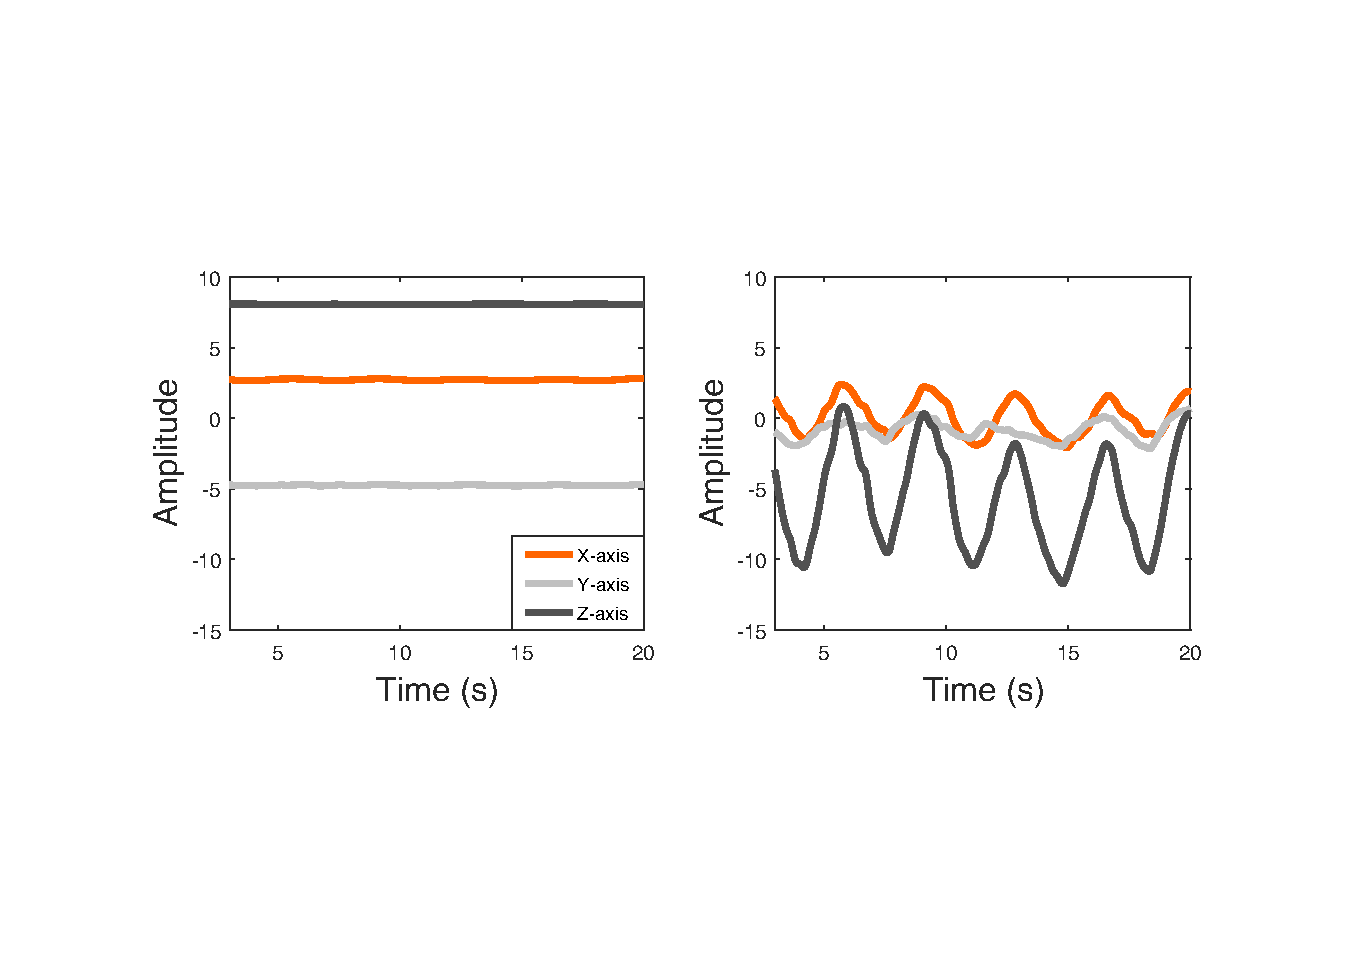
\includegraphics[width=0.48\linewidth]{Figures/cordi0.pdf}}
	\subfigure[NREM]{\label{cordi1}
		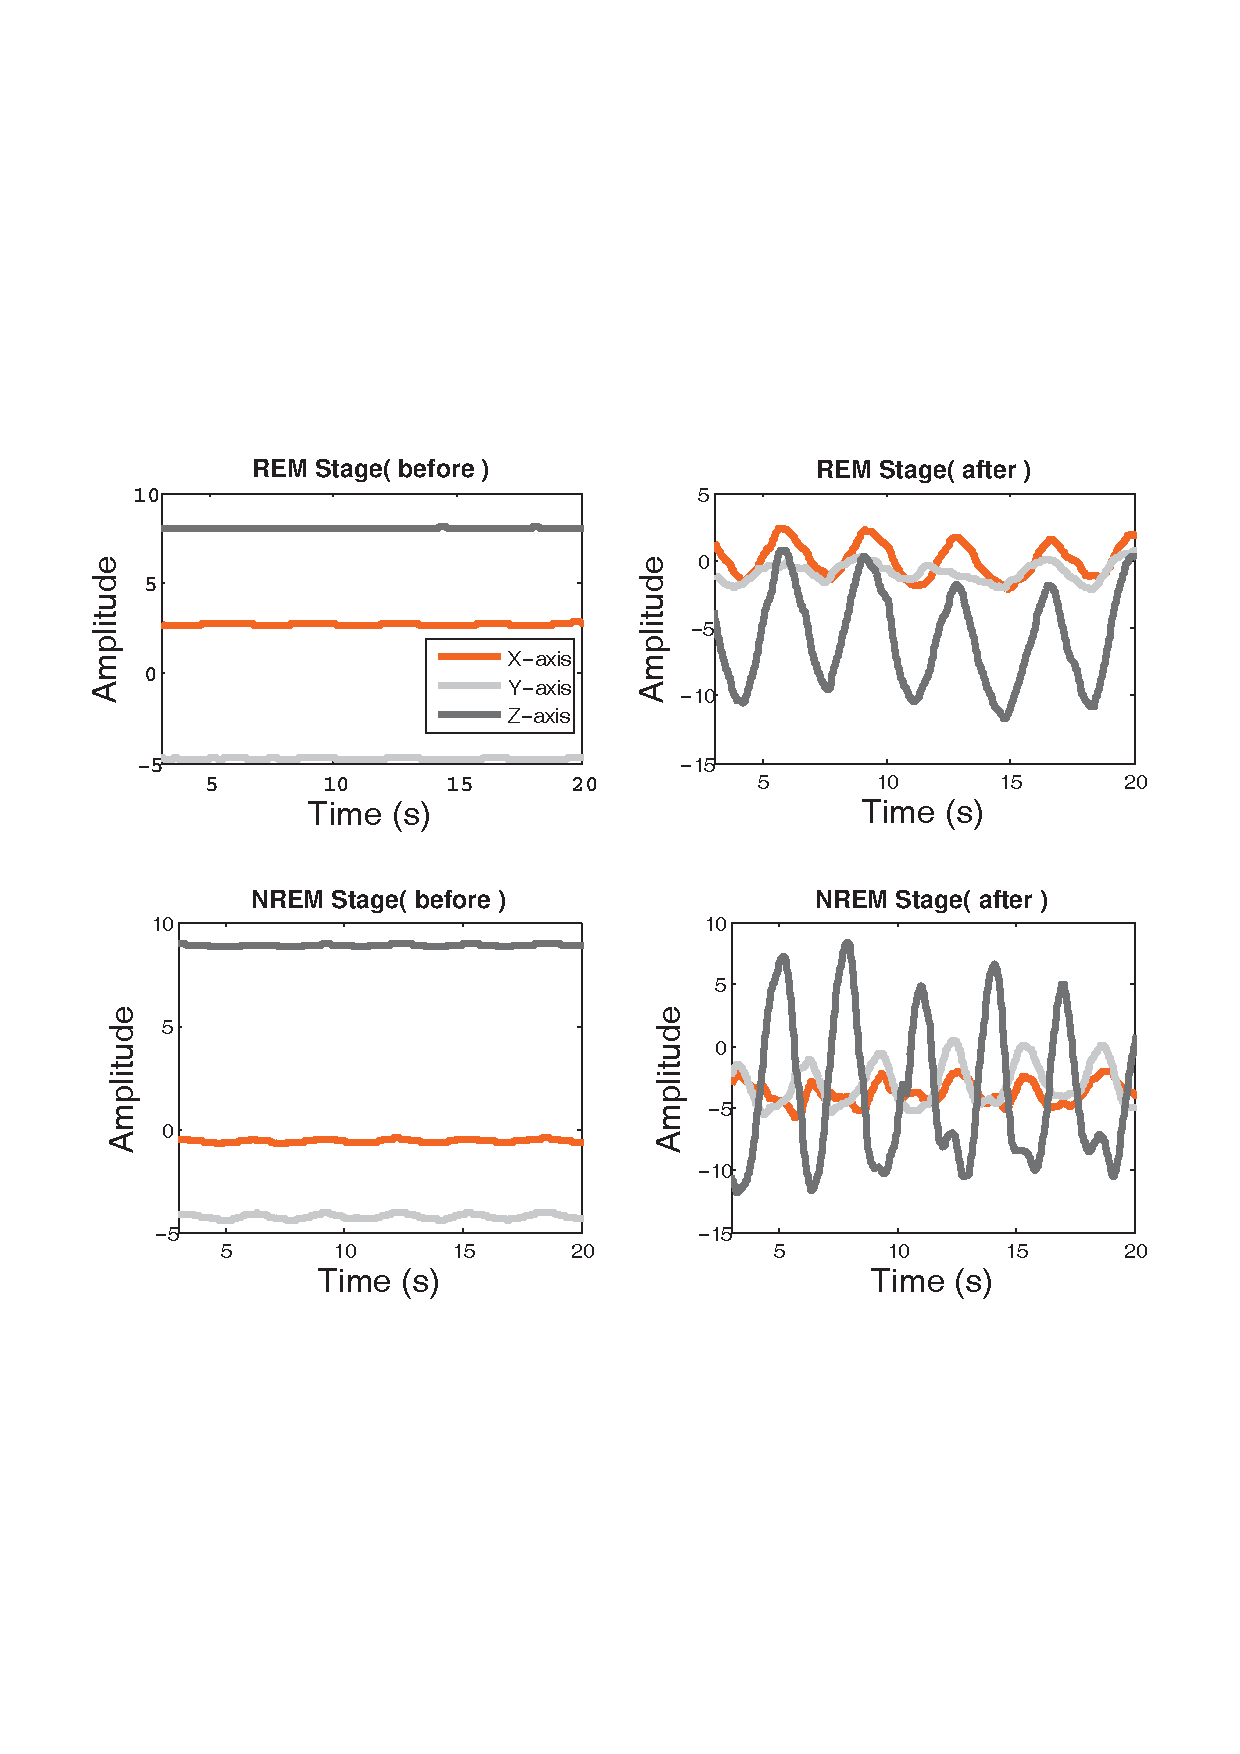
\includegraphics[width=0.48\linewidth]{Figures/cordi.pdf}}
	\caption{Acceleration data for different sleep stages.}\label{fig:cordi}
\end{figure*}

\subsection{Body Rollover Counts\label{sec:bodyrollover}}

Normally, people roll their body around 20-45 times during a sleep. The main function of body rollovers is simply to maintain a comfortable
sleeping position as maintaining the same position for a prolonged period will result in muscular tension due to the hindered blood supply,
which can also lead to local numbness~\cite{rollover2014}. Therefore, body rollovers are another key indicator of sleep quality.
{{\systemname} detects the number of body rollovers, which provides cues about sleep quality. Using the body rollover counts, \systemname
calculates the rollover frequency which is then used to identify the current sleep stage~\cite{rollover2007}}.

In general, there are six possible body rollover transitions. These include four posture transitions between the supine and laterals (left
and right), and two posture transitions between the left and right laterals. Fig.~\ref{fig:BodyRollover} depicts the case when the body
moves from the left to the right side. An intuitive way for detecting body rollover events is to estimate the rotation direction of the arm
using the rotation angle data given by the gyroscope. However, doing so is non-trivial because different users can exhibit drastically
different patterns for arm rotations; and the subtle changes in the starting arm position for the same sleeping posture could lead to a
misprediction. As an alternative to the rotation angle, we find that the tilt angles to be useful for this task because they strongly
correlate to a body rollover event. This correlation thus enables us to effectively translate the change of the tilt angle to a body
rollover event to count the occurrence of such events. Specifically, the angle values of three different axes are on the falling edge or
rising edge simultaneously during a very short time period. Fig. \ref{fig:LeftToRight} to Fig. \ref{fig:RightToLeft} show the tilt angle
reading changes under different body rollover scenarios. To this end, a na\"{\i}ve method to detect rollovers would be to rely on changes
in angle measurements. However, this method suffers a very large error since other hand movements will also induce a similar change.

\begin{figure*}[!t]
\begin{minipage}[t]{0.31\linewidth}\centering
    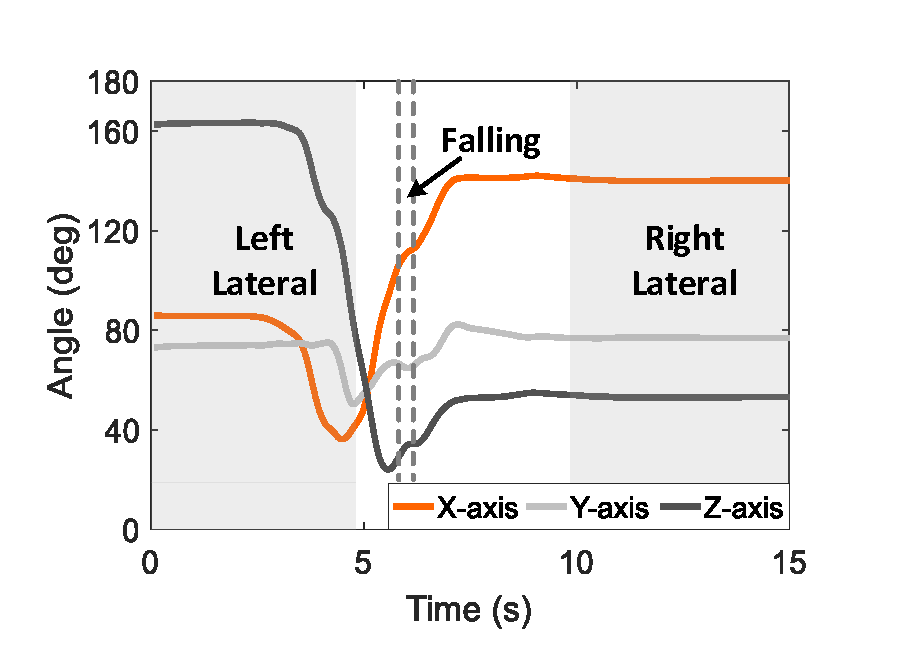
\includegraphics[width=0.97\linewidth]{Figures/LeftToRight.pdf}\centering
  \caption{From left lateral posture to right lateral posture.}\label{fig:LeftToRight}
\end{minipage}
\hspace{2pt}
\begin{minipage}[t]{0.31\linewidth}\centering
    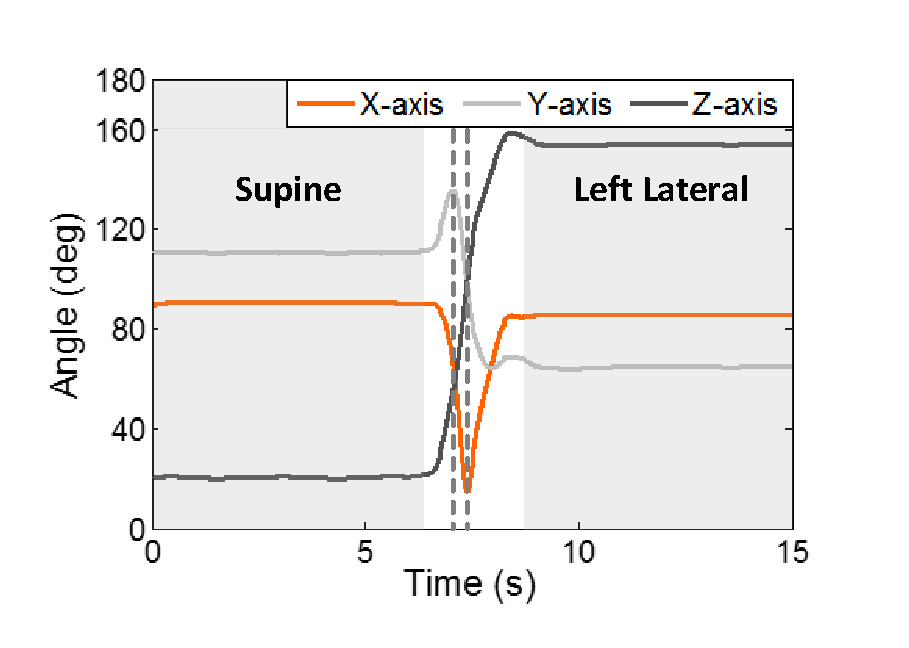
\includegraphics[width=0.97\linewidth]{Figures/SupineToLeft.pdf}\centering
  \caption{From supine posture to left lateral posture.}\label{fig:SupineToLeft}
\end{minipage}
\hspace{2pt}
\begin{minipage}[t]{0.31\linewidth}\centering
    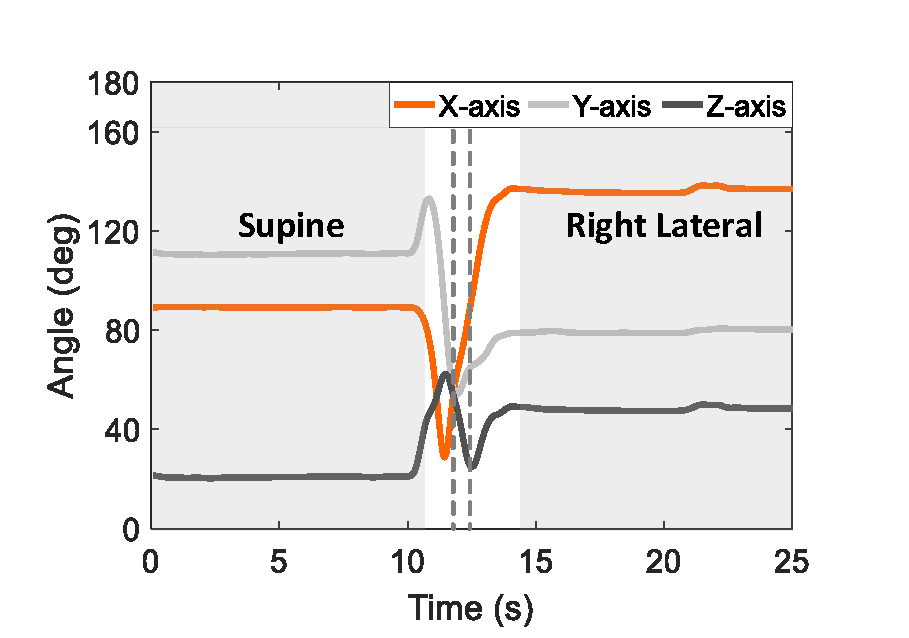
\includegraphics[width=0.97\linewidth]{Figures/SupineToRight.pdf}
  \caption{From supine posture to right lateral posture.}\label{fig:SupineToRight}
\end{minipage}
\end{figure*}

\begin{figure*}[!t]
\begin{minipage}[t]{0.31\linewidth}\centering
    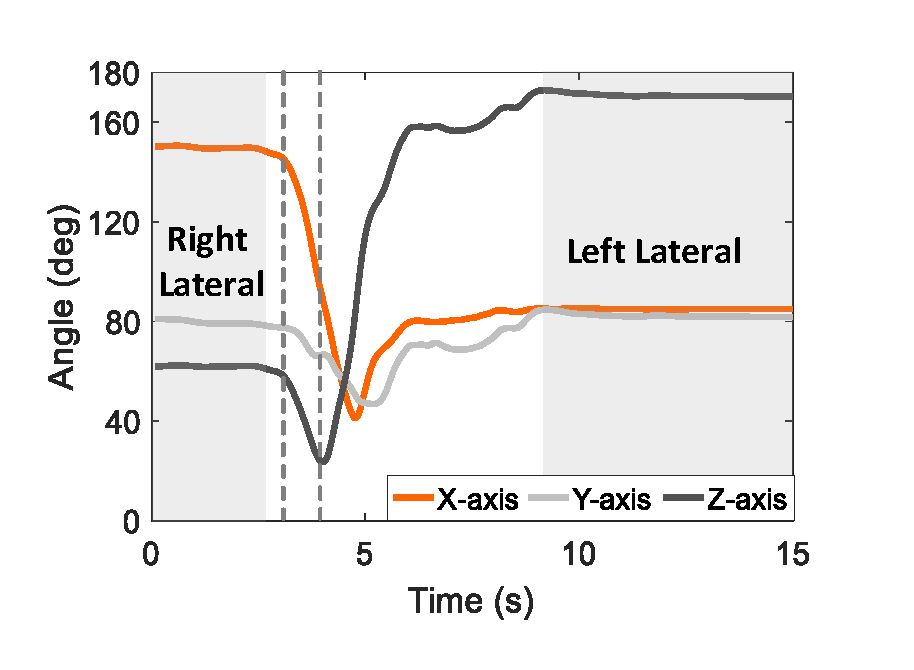
\includegraphics[width=0.97\linewidth]{Figures/RightToLeft.pdf}
  \caption{From right lateral posture to left lateral posture.}\label{fig:RightToLeft}
\end{minipage}
\hspace{2pt}
\begin{minipage}[t]{0.31\linewidth}\centering
    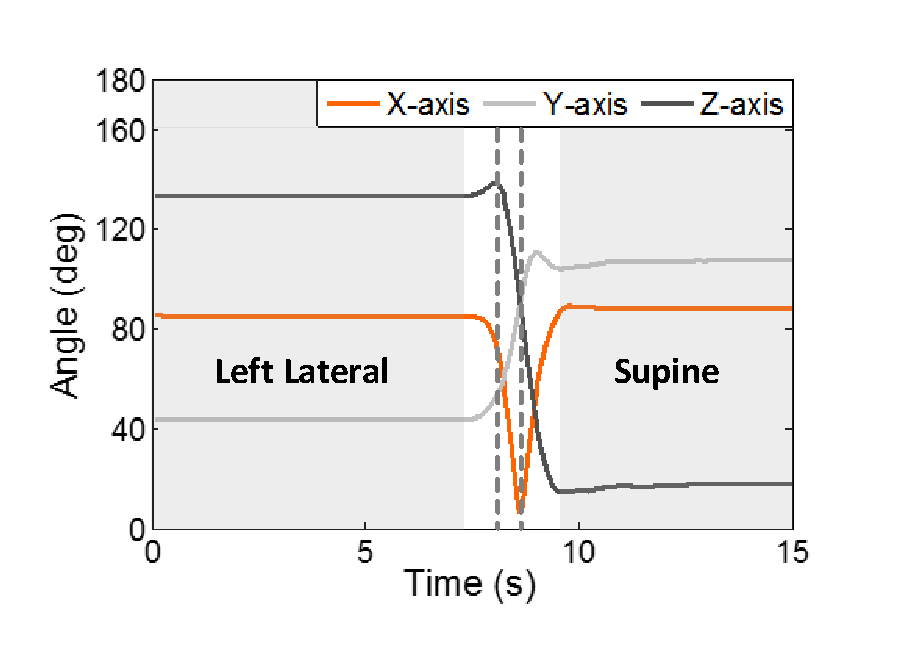
\includegraphics[width=0.97\linewidth]{Figures/LeftToSupine.pdf}
  \caption{From  left lateral posture to supine posture.}\label{fig:LeftToSupine}
\end{minipage}
\hspace{2pt}
\begin{minipage}[t]{0.31\linewidth}\centering
    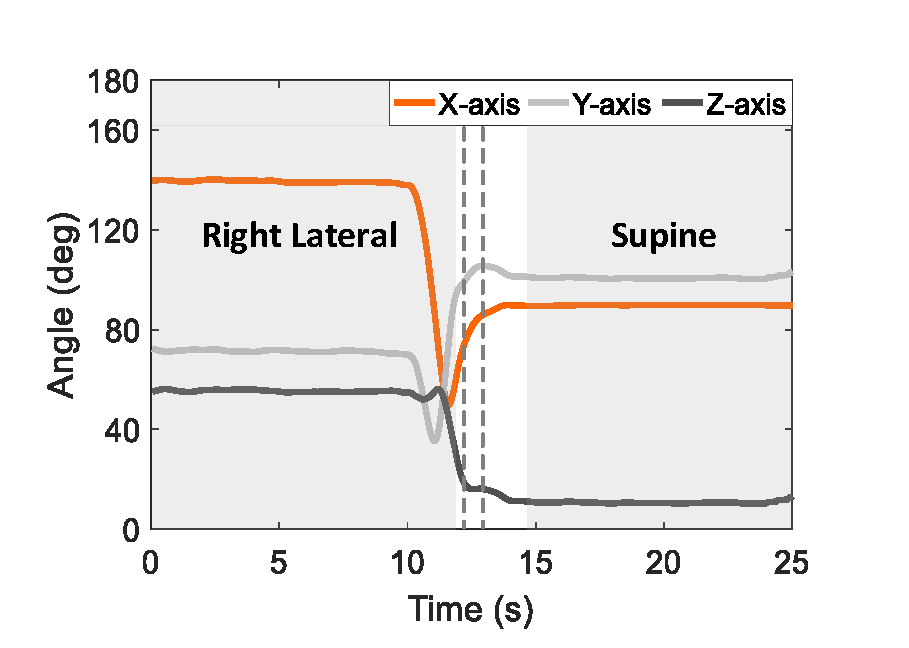
\includegraphics[width=0.97\linewidth]{Figures/RightToSupine.pdf}\centering
  \caption{From right lateral posture to supine posture.}\label{fig:RightToLeft}
\end{minipage}
\end{figure*}

To deal with this challenge, we incorporate the body postures to improve the detection accuracy. As shown in Fig. \ref{fig:BodyRollover},
the body postures are different before and after the rollover. Based on this observation, we use a two-step approach for detecting when a
body rollover took place. We first detect when the tilt angle value has changed, and mark the time the angle value was changing as when a
possible body rollover starting point. Next, we use the sleep posture classification algorithm (described in Sec.~\ref{sec:sleeppdet}) to
determine whether the body postures before (within a time window) and after (within a time window) this point were the same. If the
postures are considered to be different, our algorithm then assumes a body rollover event is detected; otherwise, it assumes the change of
tile angle readings was simply due to a changing arm position. We stress that {\systemname} not only counts the number of rollovers, but
also reports the nature of the rollover event (e.g., from which side to which side).


\subsection{Detecting Micro-body Movements \label{sec:microbo}}

Besides major-body movements, such as rollovers, there often are involuntary body movements that can affect sleep quality. With the
deepening of sleep, limbs are extremely relaxed, and a little stimulus will produce trembling and micro beating. Such behaviors are most
likely to occur during the deep sleep stage and the REM stage~\cite{ancoli2003role,Jean2000Sleep}. Therefore, by detecting such micro-body
movements and distinguish them from large-body movements can help us to further analyze the user's sleep stage. In this paper, we are
interested in the sleep-related micro-body movements including hand moving, arm raising, and body trembling.

\cparagraph{Noise canceling.} One of the challenges in detecting micro-body movements is to cancel the inherent noises brought by the
accelerometer. To cancel the noises, we apply a moving window to the collected accelerometer data points to minimize the impact of
outliers. To determine the size of the moving window, we apply different parameter settings to our training data. We found that a moving
window with a size of 35 data points gives the best average results on our training set. Therefore, we choose to apply a moving window of 35
sample points to the collected user data and then calculate the Root Sum Square (RSS) value for the data points within a window:

\begin{equation}
      Rss(t) =\sqrt{(acc_x(t))^{2}+(acc_y(t))^{2}+(acc_z(t))^{2}},
\end{equation}
$acc_x(t)$, $acc_y(t)$ and $acc_z(t)$ represent the accelerometer sample value of x-axis, y-axis and z-axis at time stamp $t$ respectively.


We can obtain the first-order derivative of from the RSS values of two consecutive time stamps, $t-1$ and $t$:
\begin{equation}
      V(t)=Rss(t)-Rss(t-1).
      \label{eq:nc}
\end{equation}

We use $V(t)$ to cancel noises in the accelerometer data. Specifically, if $V(t)$ is less than a threshold of $0.03$, we consider the
change in the RSS values is due to noises and assume there is no micro-body movement between windows $t-1$ and $t$. This threshold is
automatically learned from the training data used in our pilot study (Sec.~\ref{sec:trainingdata}).


\cparagraph{Differentiating from large-body movements.} We observe that the micro-body movement duration is often very short, lasting less
than two seconds in our training data. By contrast, the average duration for large-body movements found in our body rollover experiments
(Sec.~\ref{sec:bodyrollover}) lasts for three seconds (as shown in Fig. \ref{fig:LeftToRight} - Fig. \ref{fig:RightToLeft}). Base on this
observation, we divide the body movement events into large- and micro-body movements by measuring the signal duration time. We consider a
body movement to be micro is its duration is within two seconds; otherwise, the body movement will be labeled as a large-body movement such
as a body rollover.

\cparagraph{Distinguishing among micro-body movements.} Now we have a way to distinguish between micro- and large-body movements, we need
to identify if the detected micro-body movement is a hand movement, an arm raising action or body trembling. To differentiate among those
three micro-body movements, we turn again to consider the duration of the movement. We observe from our training data that an arm rising
action typically takes around $1.8$ second, while a hand movement and a body trembling take around $1$ second. Using the duration of the
movement, we can differentiate arm rising from the other two micro-body movements. We also find that a body trembling event tends to lead
to a more drastic change in the accelerometer readings compared to a hand movement. This observation is depicted in Fig.
\ref{fig:micro-move} using samples from one of our training users. Based on this observation, we use the change of accelerometer reading to
distinguish between the body trembling and the hand movement. Like our noise canceling strategy in Equation~\ref{eq:nc}, we do so by calculating the first-order derivative of accelerometer data to find out the peak of the acceleration data. If the peak is great than
$1.5$ and the duration of the movement took between $0.8$ and $1.2$ second, a body trembling is detected; if the peak is less than $1$ and
the duration of the movement took between $0.8$ and $1.2$ second, a hand movement is detected; otherwise, if the duration of the movement
took between $1.5$ and $2$ seconds, an arm rising is detected. These thresholds are empirically determined from our training data used in
the pilot study (Sec.~\ref{sec:trainingdata}).


\begin{figure}[!t]
\centering
      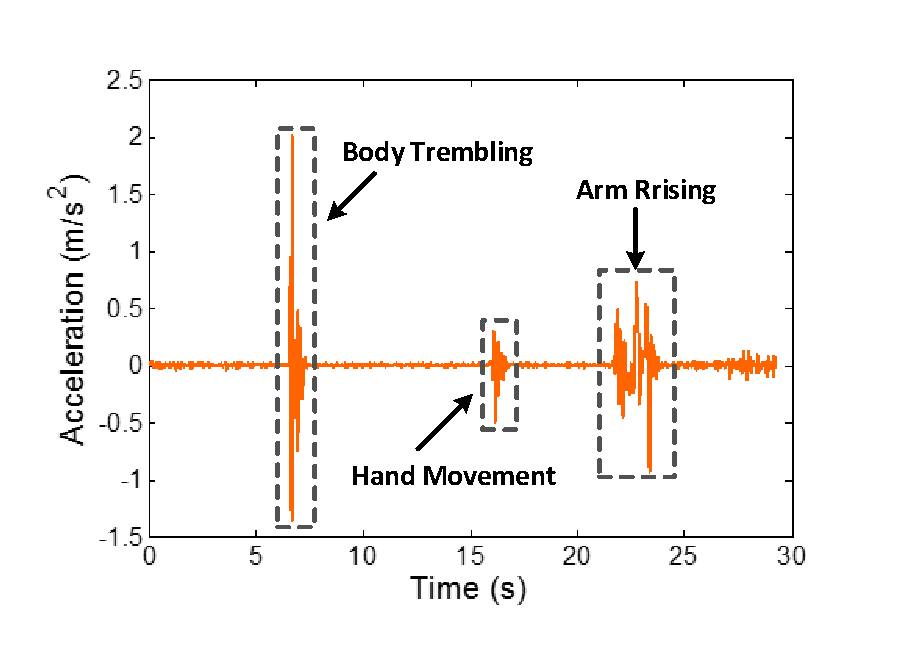
\includegraphics[width=0.43\linewidth]{Figures/Micromovement.pdf}
  \caption{Accelerometer readings for micro-body movements using samples from one of the users from the pilot study.}\label{fig:micro-move}
\end{figure}



\subsection{ Detecting Acoustic Events \label{sec:acoustic}}
Acoustic events during sleep, such as snore, cough and somniloquy, can reflect and affect user's sleep quality and physical health. For
example, the snore is one of the possible symptoms of cerebral infarction patients; and long-term snoring can also have a serious impact on
health and sleep because snoring can cause sleep apnea or narcolepsy, a sleeping disorder~\cite{snoring2016,snoring2013}. When there is a
cough, the human cerebral cortex cells are always in an excited state, limiting the depth of sleep, allowing only short sleep between
wakefulness, like many other sleep disruptions. {\systemname} is designed to detect three different acoustic events, including snore, cough
and somniloquy. \ Classical acoustic algorithms use multi-dimensional features to detect acoustic events from a complex
environment~\cite{gu2016sleep}. By contrast, we tailor our design to the problem domain to derive a simpler yet effective acoustic
detection algorithm. This is achieved by exploiting the characteristics of the different events that we target.


\begin{figure*}[!t]
\centering
 \subfigure[Six snore events.]{\label{snore}
   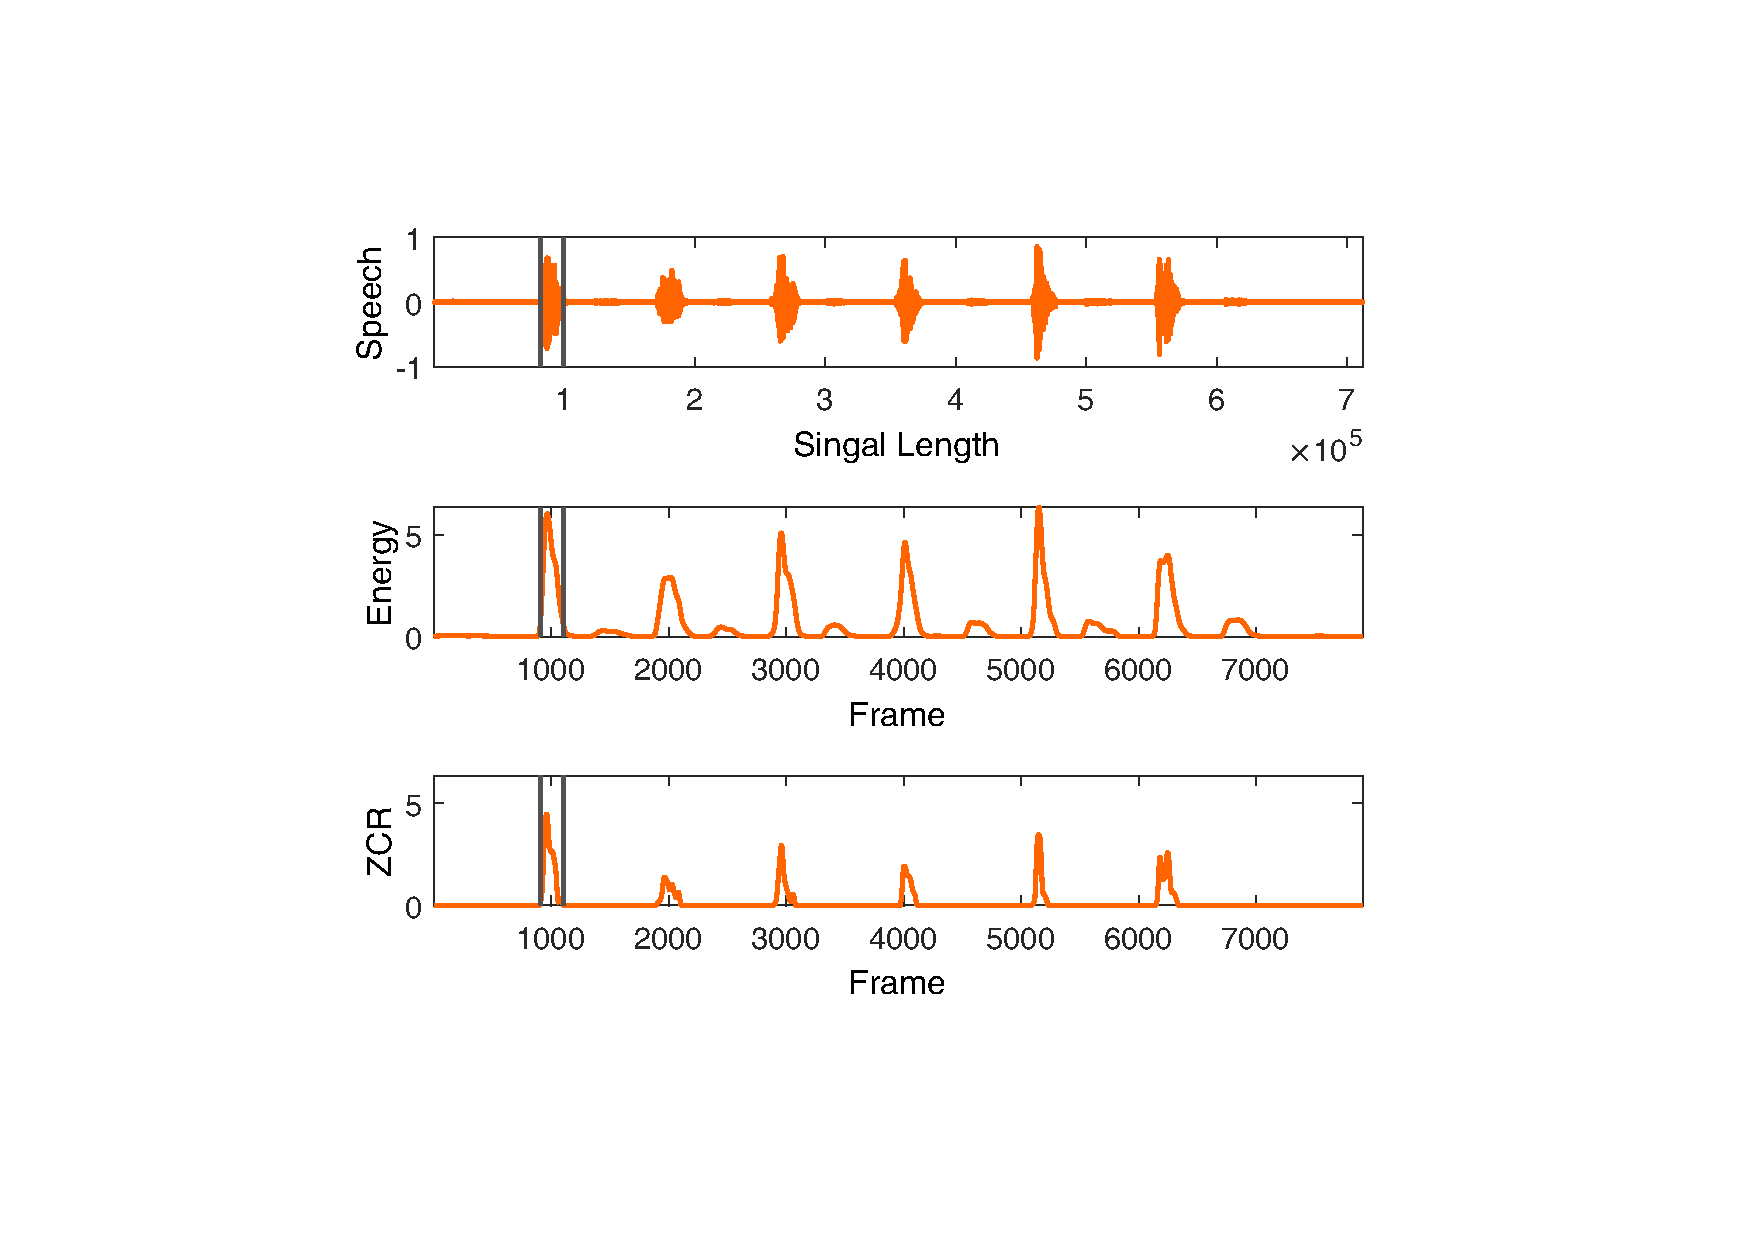
\includegraphics[width=0.32\linewidth]{Figures/snore.pdf}}
 \subfigure[Two consecutive coughs.]{\label{cough}
   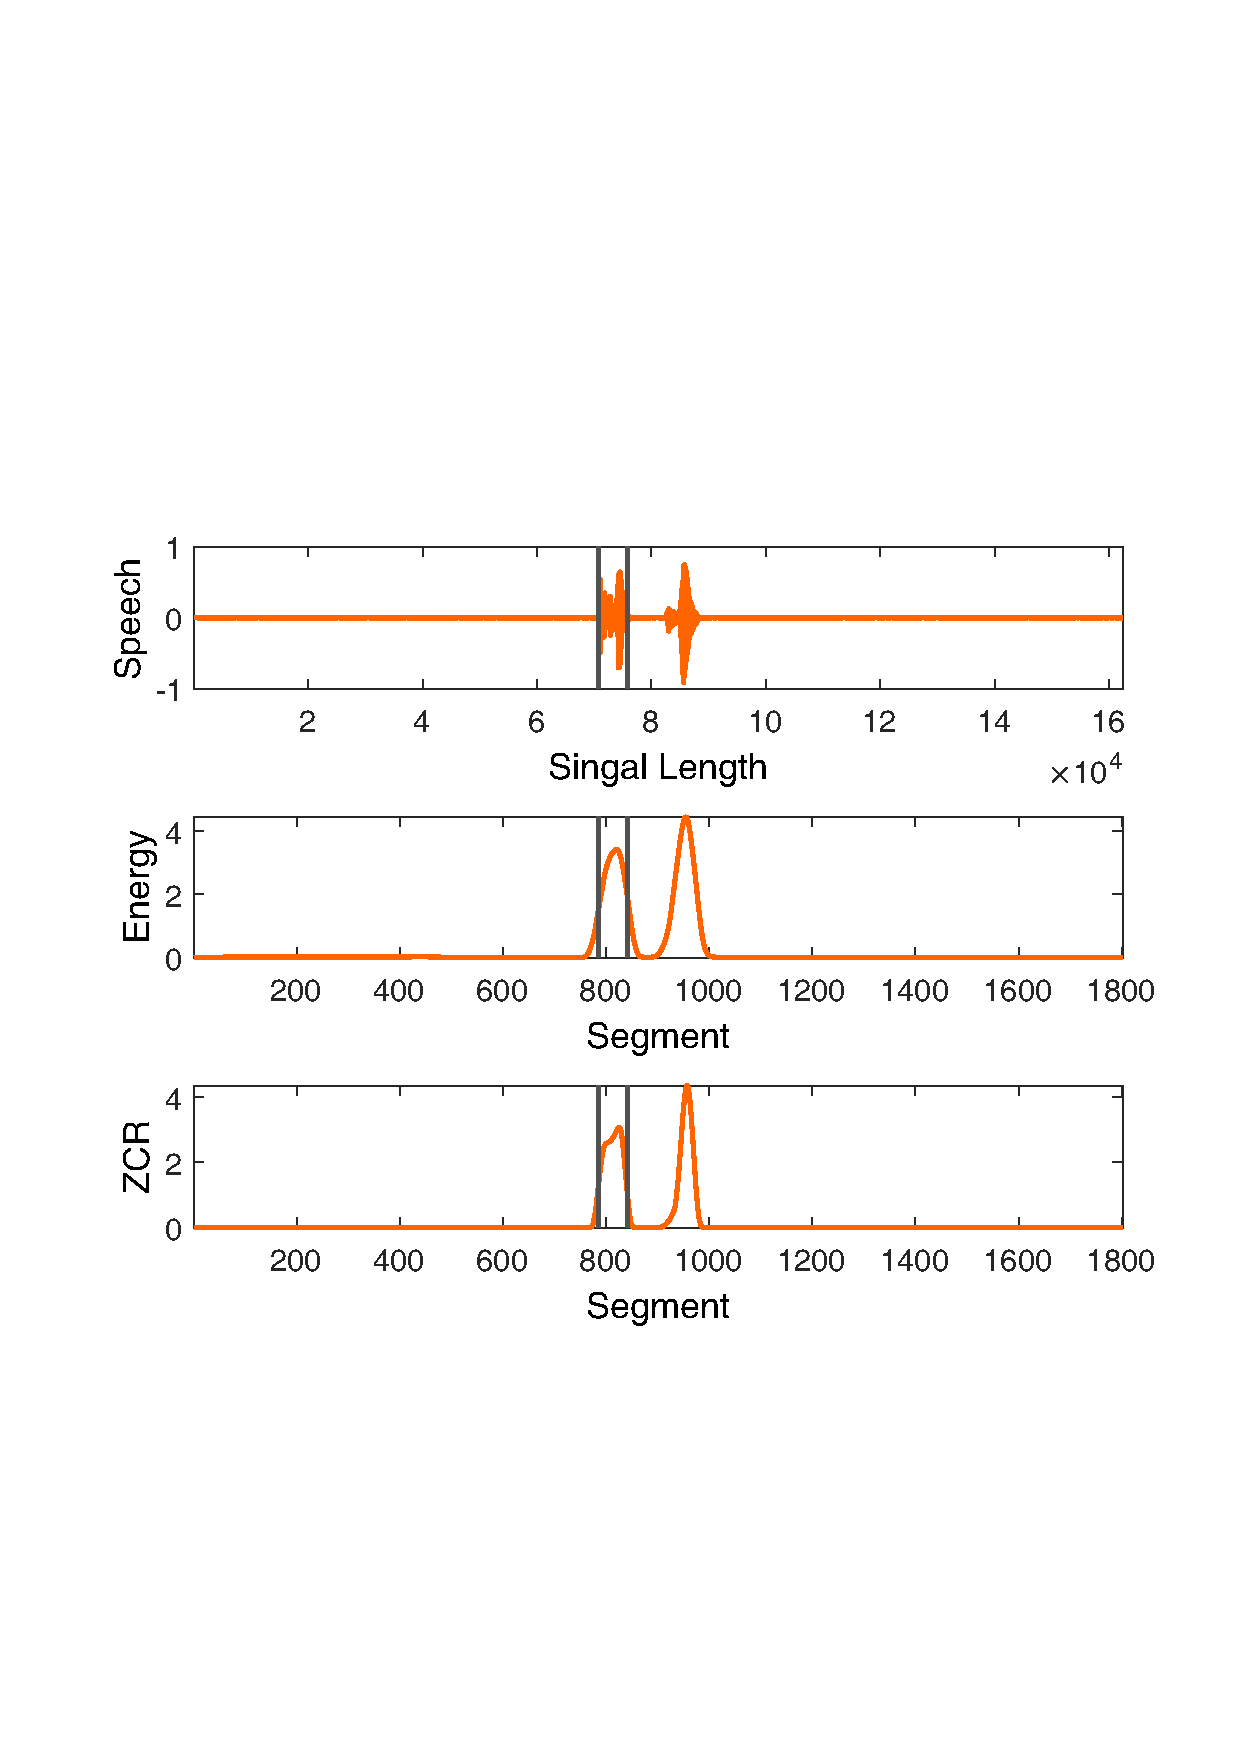
\includegraphics[width=0.32\linewidth]{Figures/cough.pdf}}
\subfigure[Somniloquy.]{\label{somniloquy}
     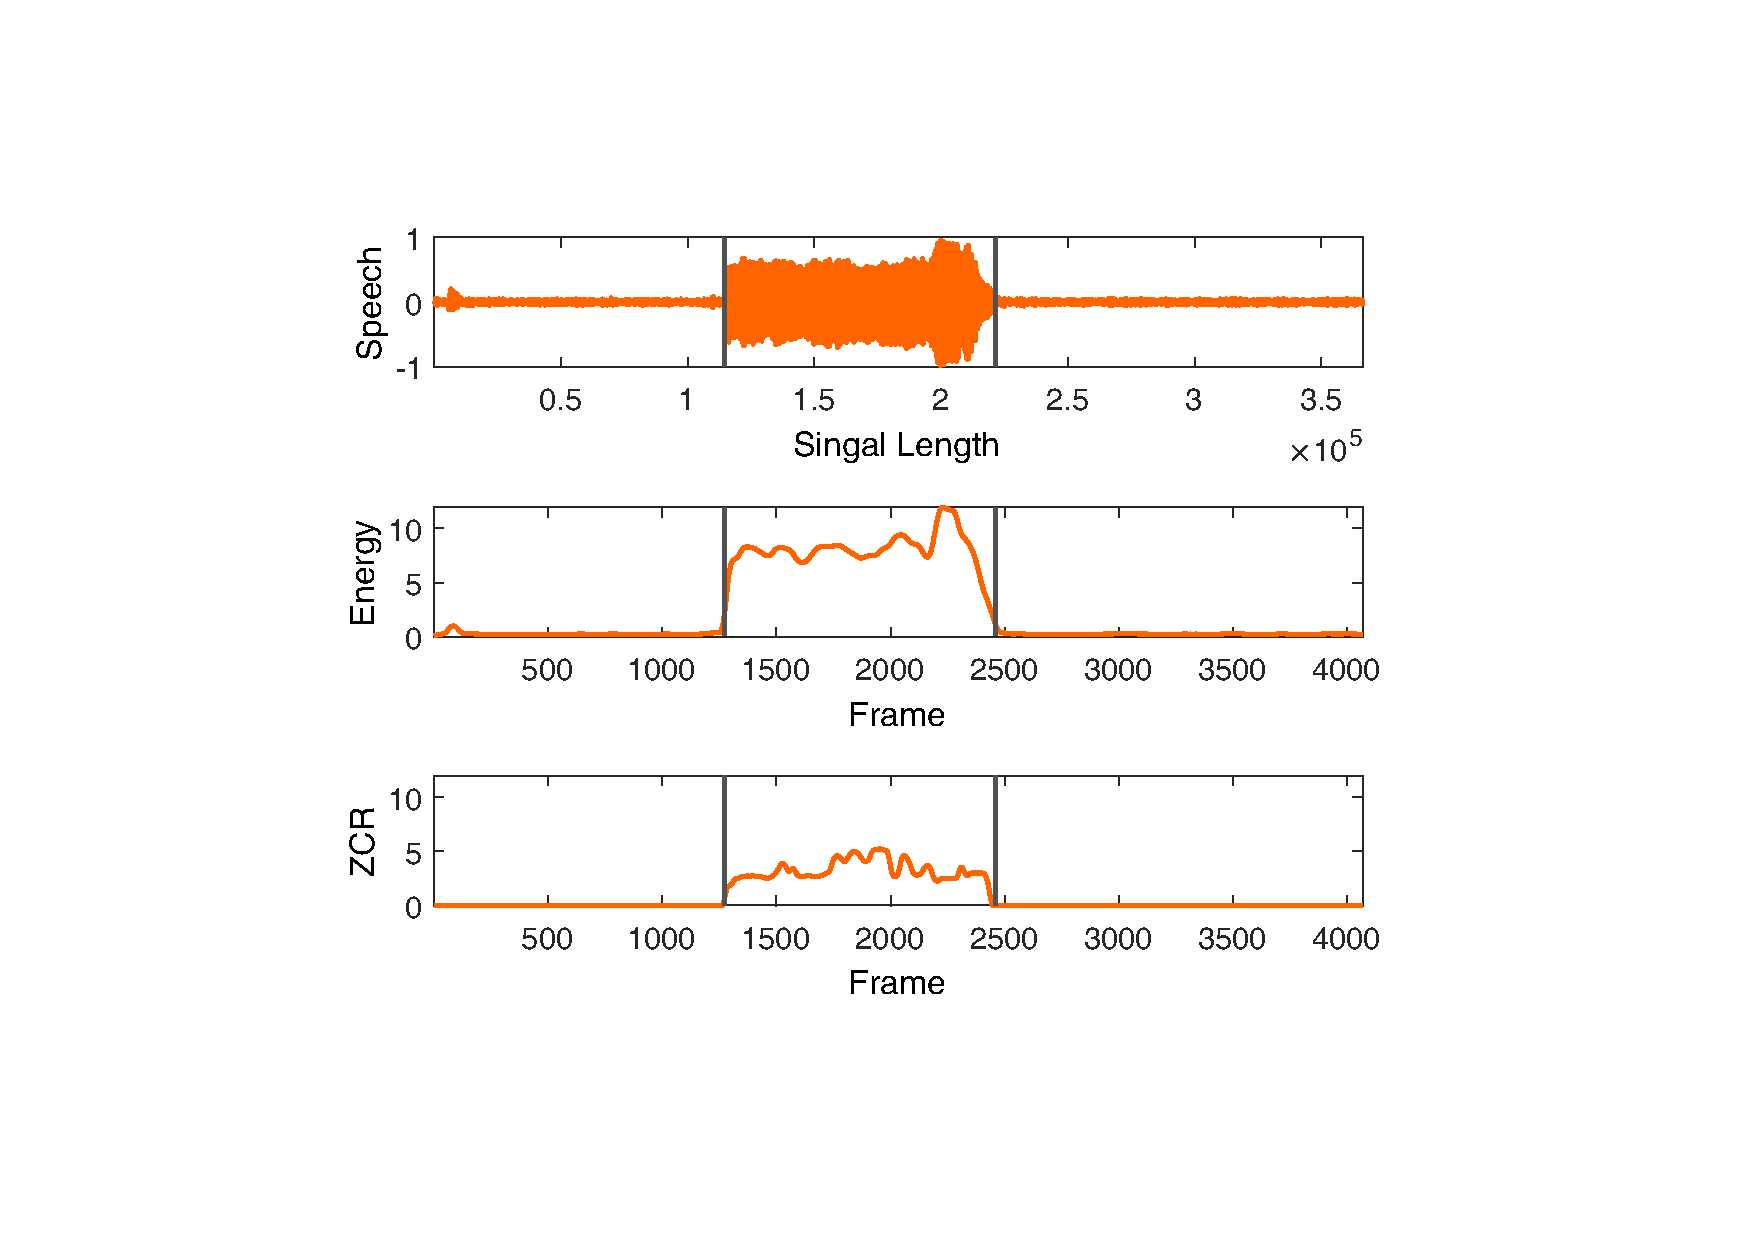
\includegraphics[width=0.32\linewidth]{Figures/somniloquy.pdf}}
\caption{Characteristics of different acoustic events targeted in this work. The thick vertical lines mark the duration of a detected acoustic event.}\label{acoustic}
\end{figure*}



\cparagraph{Acoustic event characteristics.} To understand the characteristics of the acoustic events targeted in this work,  we carry out
an interesting recognition experiment (as part of our pilot study - see Sec.~\ref{sec:trainingdata}) using the microphone built in
the smartwatch to detect the sound of people during sleep and effectively identify different acoustic events. We focus on three common acoustic
events: snore, cough and somniloquy. Ten volunteers wear the smartwatches during sleep to record the acoustic data. We manually label the
data with different acoustic events. Fig. \ref{acoustic} shows the acoustic characteristics of three events. The figure has six snore
events, two consecutive cough and somniloquy events. In the remaining paragraphs of this sub-section, we describe how to exploit these
characteristics to detect acoustic events.



\cparagraph{Pre-processing.} To identify an acoustic event, our acoustic event detection algorithm first preprocesses the recorded audio
stream by dividing it into segments of equal durations. In this work, each
 audio segment consists of 256 samples with a duration of 12 milliseconds.

\cparagraph{Observations.} Our acoustic event detection algorithm is designed based on the following observations:

 \begin{itemize}
 \item The duration a single acoustic event is different among different types of acoustic events. For example, Fig. \ref{acoustic}
     suggests that the duration of a snore is shorter than that of a cough or somniloquy. Furthermore, in general, the duration of a
     cough is shorter than that of a somniloquy signal.
 \item As shown in Fig.~\ref{acoustic}, the time intervals between two signals for two different types of acoustic events are
     significantly different. Specifically, there is a long time interval between two snores, but the time interval between two consecutive coughs is much shorter. In contrast to snores and coughs, the interval between any two consecutive somniloquy signals is irregular and does not exhibit a periodic property.
\item The frequencies for different acoustic events are significantly different. Specifically, a snore event has a continuous and periodic signal,
    while a cough or somniloquy are sudden events. As a result, the number of consecutive occurrences for coughs and somniloquy tends to
    be small during sleep.
\end{itemize}


\cparagraph{Acoustic event classification.} Our acoustic event detection algorithm is a C4.5 decision-tree-based
classifier~\cite{quinlan2014c4}. It takes as input the ``duration'', ``interval'' and ``frequency'' values of an identified acoustic event,
and predicts which of the three types acoustic events (snores, coughs, or somniloquy) the event corresponds to. The thresholds of the
decision tree are automatically learned from our pilot study training data.

To estimate the \emph{duration} of the acoustic event, we identify the start and end points of an acoustic event. After identifying the
start and end points of an acoustic event, we then perform the peak detection and use the result of peak detection to estimate the
\emph{interval} and \emph{frequency} of an acoustic event. Specifically, we use the short-term average energy (Equation~\ref{eq:shorte}) to
calculate the peak value of an acoustic signal. When the peak exceeds a pre-defined threshold, i.e., 3 dB in this work, we record the
position of each peak and calculate the \emph{interval} between two consecutive peaks. We measure the \emph{frequency} of an acoustic event
by counting the number of peaks within a time window.


%\cparagraph{Acoustic feature calculation.} % In order to identify different acoustic events accurately, we select the short-term average energy and the zero-crossing rate (ZCR) as two features.
%\textcolor{blue}{In order to identify different acoustic events accurately, we need to perform end-point detection of speech signal. So we select the short-term average energy and the zero-crossing rate (ZCR) as two features.} The short-term average energy of acoustic signal is computed as:
%
%\begin{equation}
%  E_i=\sum\nolimits_{j=-\infty}^{\infty}[x(j)\omega(i-j)]^2=\sum\nolimits_{j=i-(N-1)}^{i}[x(j)\omega(i-j)]^2,
%  \label{eq:shorte}
%\end{equation}
%
%where $N$ is the window length, $x$ is the signal and $\omega$ is the impulse response. As we can see that the short-term energy is the
%weighted sum of squared frame sample. The short-term energy can be used to distinguish the segment of unvoiced and voiced sound. It also
%can be used to differentiate the speech segment and noise segment  in  case of relatively high signal to noise ratio (SNR). The
%zero-crossing rate is computed as:
%\begin{equation}
%  Z_i = \frac{1}{2}\sum\nolimits_{j=0}^{N}|sgn[x_i(j)]-sgn[x_i(j-1)]|.
%  \label{eq:zeroc}
%\end{equation}
%
%
%where $Z_i$ indicates how often (i.e., the number of times) the acoustic signal waveform passes through the horizontal axis (zero level).



\cparagraph{Determining the start and the end points.} Traditional end-point detection algorithms~\cite{endpoint2008} are
ill-suited to our problem. This is because they typically use a fixed threshold which must be obtained by examining a large number of data
samples. As a result, a traditional end-point detection algorithm has two drawbacks. Firstly, a fixed threshold is highly unlikely to be
optimal for different users (due to different sleep patterns) and environments (due to different environmental noises). Secondly, using a
large number of data samples to determine the threshold incurs significant overhead for data collection.


To address the two drawbacks of traditional end-point detection algorithms, we develop a novel method based on the short-term energy and
the zero-crossing rate (ZCR). Our method requires significantly fewer data samples to determine the optimal threshold on a per user
per-environment basis.

The short-term average energy of an acoustic signal is computed as:

\begin{equation}
  E_i=\sum\nolimits_{j=-\infty}^{\infty}[x(j)\omega(i-j)]^2=\sum\nolimits_{j=i-(N-1)}^{i}[x(j)\omega(i-j)]^2,
  \label{eq:shorte}
\end{equation}

where $N$ is the window length, $x$ is the signal and $\omega$ is the impulse response. As we can see that the short-term energy is the
weighted sum of squared frame sample. The short-term energy can be used to distinguish the segment of unvoiced and voiced sound. It also
can be used to differentiate the speech segment and noise segment  in  case of relatively high signal to noise ratio (SNR).


The zero-crossing rate is computed as:

\begin{equation}
  Z_i = \frac{1}{2}\sum\nolimits_{j=0}^{N}|sgn[x_i(j)]-sgn[x_i(j-1)]|.
  \label{eq:zeroc}
\end{equation}


where $Z_i$ indicates how often (i.e., the number of times) the acoustic signal waveform passes through the horizontal axis (zero level).



%
% may cause error detection at the beginning of an acoustic event. Second, the
%requirement of a large number of data samples would lead to large system latency. To address these issues, we develop a detection method
%that does not require pre-sampling to obtain the optimal thresholds. Instead, our algorithm estimates the thresholds on a per signal basis.
%This strategy not only reduces the number of data samples needed, but also leads to a higher accuracy.
%
Our algorithm works as follows.  Since the first and last few audio segments are mostly mute or are background noises, we select the first
and last five segments to calculate their short-term energy, which is denoted as $E_s$ and $E_e$ respectively for the first and last
segments. The two energy values are then combined to obtain the mean, $E_n$, as the estimated energy value of noise segments. Let the
maximum value of the short-term energy over all segments denoted as $\max (E)$. Then, the average short-term energy, $DE$, is given as:
\begin{eqnarray}
      &E_n = \frac{(E_s+E_e)}{2}, \\
      &DE = \max (E)-E_n.\label{eq:DE}
\end{eqnarray}

We can use $EH$ and $EL$ to represent the high and the low thresholds respectively for short-term energy as:
\begin{eqnarray}
      &EH=\alpha \times DE+E_n,\\
      &EL=\beta \times DE+E_n,
\end{eqnarray}
where $\alpha$ and $\beta$ are the multiplier factors of an energy value, $DE$.


Here, we need to choose the right values for coefficients $\alpha$ and $\beta$ to ensure that we can accurately detect the start and end
points of a speech signal. To that end, we use the night time sound data from our training dataset to determine $\alpha$ and $\beta$.
Specifically, we tested $\alpha$ with values ranging from 0.1 to 0.5, and $\beta$ with values ranging from 0.01 to 0.09. We found that
setting $\alpha$ to  0.1 and $\beta$ to  0.06 gives the best overall results in our training dataset.

To minimize the impact of occasionally happened noises, we set the minimum length of the signal segment and measure the duration of the
signal when searching for the start and end points. If the length of an acoustic signal is less than the minimum, the signal segment is
considered to be a noise segment.

\cparagraph{Example.} As an example, the two thick vertical lines in Fig. \ref{acoustic} mark a detected acoustic event. The start and end
points are used to calculate the duration of an event, as well as the interval between two consecutive acoustic events. To measure the
frequency, we count the number of peak points of an acoustic event signal. By feeding the values of the ``duration", ``interval" and
``frequency", our decision-tree-based acoustic detection algorithm can then predict which type of events an acoustic signal corresponds to.



\subsection{Tracking Illumination Conditions \label{sec:illumination}}
Studies have shown that there is a significant interaction between the illuminance level and the mental state of the individual
\cite{light77}. For example, the bright light can counteract subjective fatigue during the daytime, but at night it will seriously disrupt
sleep. Too much light exposure can shift our biological clock, which makes restful sleep difficult to achieve, it affects our sleep and
wake cycle \cite{light2007}.  Besides, we also note that the dim light will affect our sleep too. According to a previous study
\cite{light2016}, the dim artificial light during sleep is significantly associated with the general increase in fatigue, and the proper
light can be used to increase the sense of exhaustion and promote sleep. Therefore, the illumination condition in a sleeping environment
has a significant impact on sleep.

{\systemname} uses the ambient light sensor to detect the illumination condition during sleep. We visit the bedroom of our ten pilot-study
users at night and use the ambient light sensor to test the lighting conditions in the bedroom. We find that in the absence of lights in
the bedroom, the light sensor reading is between 1 Lux to 4 Lux. In some cases, the light of the smartwatch screen can raise the light
sensor reading to 4 Lux when the bedroom is dark. In other cases, when the bedroom has weak lights (e.g., when the bedroom is illuminated
using a table lamp), the light sensor's average readings are below 10 Lux. Based on these observations, we divide the illumination
intensity of the bedroom into two categories. When the bedroom has weak lights (i.e., the light sensor reading is no greater than 10 Lux),
and when the bedroom has strong lights (i.e., the light sensor reading is greater than 10 Lux). Using the threshold of 10 Lux, we can then
map the light sensor readings to one of these two groups.


However, the light sensor may be obscured, which leads to large errors in measuring the illumination level. For example, a user's
smartwatch may be covered under the quilt when he/she turned over unconsciously, and thus the illumination readings on the smartwatch may
not reflect the real lighting situation. Most of the previous works on smartphone-based light detection have used the proximity sensor to
detect whether the light sensor is blocked or not. However, such an approach is not applicable to the off-the-shelf smartwatches because
they typically do not have a proximity sensor.  The key to dealing with this practical challenge is that the illumination would drop suddenly
when the smartwatch is covered by other objects. There are two possibilities for the sudden drop in light intensity. For most smartwatches,
the light sensors are usually installed in the front face of it. The first case is the indoor lighting facilities are closed. The second
case is the wrist turned so that the back of the hand become downward, thus blocking the light sensor in front of the smartwatch. Such a
situation often happens in real life. For examples, when a user changes the sleeping posture to the left side, his/her hand may be close to
the pillow with the palm facing up; or the back of the hand may become downward because of a hand movement. To avoid this erroneous
illumination condition measurement, we detect whether the user is performing a wrist flip over a period of time during the intensity
plummeting. We detect the wrist flip based on two aspects: (i) the rotation angle of the smartwatch; (ii) whether the light intensity
maintains stable after the sharp drop. If the wrist flips, we use the average of the previous light intensity as the intensity of the time
period. It should be noted that, because the illumination condition detection algorithm is relatively simple, it is not explained in the
experimental part.

\subsection{Sleep Stage and Quality}

Sleep is generally considered as a cyclical physiological process composed of three stages: rapid eye movement (REM) stage (see also
Sec.~\ref{sec:labelrem}), light sleep stage and deep sleep stage. REM is an active period of sleep marked by intense brain activities and
dream occurrence. Light sleep stage is a period of relaxation, when the heartbeat, breathing rate and muscle activity slow down. Deep sleep
stage triggers hormones to promote body growth, as well as the repair and restoration of energy.  The biological characteristics of
different sleep stages exhibit distinguishingly.

In the clinical sleep study, the sleep stages are mainly identified by simultaneously evaluating three fundamental measurement modalities
including brain activities, eye movements, and muscle contractions. The EEG measure using electrodes placed around the scalp interpret
various sleep/wake states of the brain. Moreover, EMG and EOG using electrodes placed on the skin near the eyes and on the muscles,
respectively, measures in deeply differentiating REM stage from all the other stages. However, apart from the implicit physiological
activities, sleepers usually exhibit distinguishable physical activities in different sleep stages. For example, there are somniloquy and
body trembles caused by frequent dreams generally appear in REM, large body movements such as body rollovers and arm raising happen in
light sleep and micro-body movements such as body trembling and snoring occur in deep sleep.  In the meanwhile, the breathing amplitude in
NREM stage is larger compared with the REM stage. Moreover, the sleep cycle usually repeats four to six times over a sleep. The sleeper
usually experiences a transition from light sleep to deep sleep and then enters REM, but sometimes there is also possible a phenomenon of
skipping some certain sleep stages occurs during sleep. However, despite this, the dependence between two successive sleep stages still
exists and different sleep stages have potential conversion probabilities, which also mentioned in Sleep Hunter \cite{gu2016sleep}.

To separate between these states, we build a Hidden Markov Model~\cite{johnson2010hidden} for identifying the current sleep stage of the
user. As the input, i.e., the observed states, we use a series of detected sleep events and the sleep stage sequence is modelled as a
hidden state, i.e., $obs_t$=($NB(t),NB_M(t),BA(t),NA(t)$) represent the feature vector at the detection phase $t$. The explanation of each
item, which is the input of HMM, is listed as follows. $NB(t)$: the number of occurrences of body rollover during the detection phase t.
$NB_M(t)$: the number of occurrences of micro-body movement. $BA(t)$: the measurement of respiratory amplitude.  $NA(t)$: the number of
occurrences of the acoustic events. The $states_t$ =$\{$light sleep; deep sleep; REM$\}$ is an output of our model, which represents the
sleep stage in the detection phase $t$. In the training of the HMM model, we use nocturnal sleep data from 10 volunteers who participated
in the pilot study. We use the sleep-related events of the 10 volunteers as observation sequences and the corresponding sleep stages
detected by Fitbit as hidden state sequences, to generate HMM models. Specifically, we first use the maximum likelihood estimation method
for parameter estimation, the state transition matrix and the confusion matrix; we then use the Viterbi algorithm~\cite{anguera2012speaker}
to acquire a series of implicit state sequences corresponding to the observed sequences.  As a result, we can estimate the sleep stage
during a time window. Finally, we can get the durations of all sleep stages over the whole sleep process.

Further, to quantize the sleep quality, we use the Sleep Quality Report model introduced in \cite{gu2016sleep}. Let $SQ$ be the value of the sleep quality, then $SQ$ is given as follow:
 \begin{equation}
SQ=\frac{(REM \times 0.5+Light \times 0.75+Deep) \times 100}{REM+Light+Deep}
 \end{equation}
where, REM, Deep and Light represent the duration time in a sleeping process. The range of $SQ$ is from 50 to 100. A high value of $SQ$
shows a better  sleep quality.
